\documentclass[12pt, a4paper]{article}

% ── Packages ────────────────────────────────────────────────────────────────
\usepackage[margin=1in]{geometry}
\usepackage{mathptmx}       % Times New Roman (drop-in replacement for times.sty)
\usepackage{setspace}
\usepackage{titlesec}
\usepackage[hidelinks]{hyperref}
\usepackage[round, authoryear]{natbib}   % APA-style citations
\usepackage{graphicx}
\usepackage{booktabs}
\usepackage{array}
\usepackage{enumitem}
\usepackage{longtable}
\usepackage{microtype}
\usepackage{xcolor}
\usepackage{tikz}
\usetikzlibrary{arrows.meta}

% ── Typography ───────────────────────────────────────────────────────────────
\onehalfspacing
\setlength{\parskip}{6pt}
\setlength{\parindent}{1.5em}

% ── Section formatting ────────────────────────────────────────────────────────
\titleformat{\section}{\large\bfseries}{\thesection.}{0.5em}{}
\titleformat{\subsection}{\normalsize\bfseries}{\thesubsection}{0.5em}{}
\titleformat{\subsubsection}{\normalsize\itshape}{\thesubsubsection}{0.5em}{}

% ── Metadata ─────────────────────────────────────────────────────────────────
\title{\textbf{A Neuroscience-Grounded Framework for Cognitive Self-Governance: \\
       Source Monitoring, Metacognitive Architecture, and \\
       Systematic Skill Training} \\[0.5em]
       \large \textit{Preprint --- Submitted for Expert Review}}

\author{[Author contact withheld for blind review]\\[0.3em]
        \small Correspondence: \textit{[withheld for review]}}

\date{March 2026}

% ─────────────────────────────────────────────────────────────────────────────
\begin{document}

\maketitle
\thispagestyle{empty}

% ── Abstract ─────────────────────────────────────────────────────────────────
\begin{abstract}
\noindent
Cognitive self-governance --- the capacity to detect and attribute the origins of
one's own thoughts, beliefs, and emotional states before acting on them --- is
trainable in principle but lacks a neuroscience-grounded systematic development
framework. This preprint presents the \textit{Mental Mastery} framework: a
three-layer, 41-skill taxonomy reviewed against 33 peer-reviewed papers. The layered
sequence is neurologically motivated: Layer~2 metacognitive monitoring requires
Layer~1 interoceptive and attentional signal quality as necessary input; Layer~3
intentional pattern modification requires Layer~2 monitoring reliability as a
safety precondition. The Self-Boundary Integrity domain is grounded in source
monitoring theory \citep{johnson1993, mitchell2009, simons2008}, identifying five
failure modes --- source amnesia, misattributed familiarity, cryptomnesia,
fiction-as-fact incorporation, and criteria relaxation under load --- as the
principal training targets. Two critical empirical constraints are incorporated:
the stress-transfer problem \citep{raio2013} (prefrontal strategies trained under
calm conditions show zero transfer to acute physiological arousal) and the
domain-specificity of metacognitive accuracy \citep{morales2018, fleming2014}
(monitoring does not transfer across domains; each requires independent training
and assessment). The central hypothesis --- that sequential development of
interoceptive and attentional substrates, followed by domain-specific metacognitive
monitoring training, produces measurably improved source attribution accuracy
under load in healthy adults --- is currently untested as a composite architecture.
We present the framework as a structured, mechanistically motivated research
programme and invite expert review of the mechanistic claims, assessment design,
and safety provisions.

\medskip\noindent
\textbf{Keywords:} metacognition; source monitoring; neuroplasticity; cognitive
self-governance; mindfulness-based training; interoception; prefrontal cortex;
probabilistic monitoring architecture; stress-inoculation; domain-specificity
\end{abstract}

\newpage
\tableofcontents
\newpage

% =============================================================================
\section{Introduction}
% =============================================================================

A practitioner who consistently detects shifts in their own cognitive state --- arising
from framing effects, social influence, narrative exposure, or emotional contagion ---
before those shifts complete demonstrates measurably enhanced monitoring reliability
under load compared with untrained individuals. The question of whether this monitoring
capacity is systematically trainable, and if so how, is both a scientific and a
practical one. Exposure conditions that activate documented source monitoring failure
modes --- repeated framing, narrative embedding, arousal-mediated criteria relaxation,
and fluency-based familiarity effects --- are well-characterised mechanisms through
which information environments exploit known gaps in human source attribution
\citep{johnson1993}. The capacity to resist these influences depends on
cognitive skills that, while trainable in principle, have no systematic development
framework grounded in neuroscience.

Existing mindfulness-based interventions (MBIs), though well-studied, are developed
primarily as therapeutic tools for stress reduction, depression relapse prevention,
and attention regulation \citep{gkintoni2025, calderone2024}. They were not designed
to produce cognitive self-governance in the specific sense developed here: the
real-time detection and attribution of the origins of one's own thoughts, beliefs,
and emotional states, maintained under conditions of social pressure, emotional
activation, and physiological arousal. The result is that while MBI evidence is
relevant and is drawn upon extensively in this framework, it cannot simply be adopted
wholesale. Key findings --- including the stress-transfer problem \citep{raio2013},
the domain-specificity of metacognitive accuracy \citep{morales2018, fleming2014},
and the behavioural relevance gate for neuroplasticity \citep{fallon2009,
beyeler2017} --- substantially constrain what MBI training produces and what
additional training is required.

\medskip\noindent
\textbf{Central hypothesis:} \textit{Sequential development of interoceptive
accuracy and attentional stability, followed by domain-specific metacognitive
monitoring training, produces measurably improved source attribution accuracy
under cognitive and physiological load in healthy adults.}
\medskip

This hypothesis is currently untested as a composite architecture. Each
component --- interoceptive accuracy training, emotion granularity development,
metacognitive monitoring, origin monitoring, stress-inoculation, and pattern
interruption --- has independent partial empirical support, detailed in
Section~3. The combinatorial interaction: whether these components, trained in
the specified sequence and at the specified depth, produce an integrated capacity
greater than the sum of individually-trained components, has not been studied.
The Mental Mastery framework is accordingly presented as a \textbf{structured,
mechanistically motivated research programme, not an established intervention}.
Its contribution at this stage is to specify the hypothesis precisely enough
that it can be tested, and to do so in a form that is internally consistent with
the neuroscience at the component level.

This preprint presents the Mental Mastery framework: a 41-skill taxonomy organised
into three functional layers and nine domains, reviewed against 33 peer-reviewed
papers. Section~2 describes the framework's architecture. Section~3 provides the
neuroscientific foundation for each core mechanism. Section~4 justifies the
three-layer sequence as neurologically non-arbitrary. Section~5 grounds the
probabilistic monitoring architecture in source monitoring theory and documents its structural
limits. Section~6 describes critical design constraints that emerged from the
evidence review. Sections~7--8 describe training and assessment design. Section~9
addresses individual differences. Section~10 states honest boundaries. Section~11
summarises convergence across the 33 papers. Section~12 concludes, and an
unnumbered section presents a formal request for expert review.

\paragraph{What this framework does not claim.}
The language of ``source attribution'' and ``cognitive self-governance'' risks
ideological projection if its scope is not explicitly bounded. The framework
makes no claim to:
\begin{enumerate}[leftmargin=2em]
\item \emph{Epistemic immunity.} Trained practitioners do not become resistant
to error or manipulation. Source attribution accuracy improves probabilistically
--- failure modes remain possible under sufficient load, deception sophistication,
or individual biological constraints. The framework trains a skill; it does not
install a filter.
\item \emph{Bias elimination.} The training does not reduce motivated reasoning,
confirmation bias, or identity-protective cognition. Those mechanisms operate at
the level of goal-directed evaluation, downstream of the encoding and attribution
processes the framework targets. Improving source attribution accuracy does not
make practitioners less partial; it makes the origins of their partiality more
attributable.
\item \emph{Value superiority.} The framework is indifferent to belief content.
No value system, political position, or belief structure is more or less
``correctly monitored'' than any other. The training targets the process of
attribution, not the outputs of evaluation.
\item \emph{Political neutrality guarantees.} Political preferences, partisan
reasoning, and ideological commitments are not targets of source monitoring
training and are not predicted to change. The framework has no claim on what
practitioners should believe or how they should evaluate contested questions.
\end{enumerate}
The framework is a metacognitive skill development programme. Its primary outcome
is source attribution accuracy under load. Everything else --- including how
practitioners apply that accuracy --- is outside the framework's scope.

% =============================================================================
\section{Framework Architecture}
% =============================================================================

The framework is organised into three layers and nine domains, with four cross-layer
skills (Table~\ref{tab:architecture}).

\begin{table}[htbp]
\centering
\caption{Framework Architecture: Three Layers, Nine Domains, 41 Skills}
\label{tab:architecture}
\small
\begin{tabular}{llcp{6cm}}
\toprule
\textbf{Layer} & \textbf{Domain} & \textbf{N} & \textbf{Representative Skills} \\
\midrule
L1: Foundational & Somatic Intelligence & 4 &
  Sensation Recognition, Interoceptive Accuracy, Physiological Baseline Mapping, Arousal Detection \\
L1: Foundational & Emotion Granularity & 4 &
  Primary Identification, Somatic-Emotion Mapping, Vocabulary Expansion, Gradient Detection \\
L1: Foundational & Attention & 5 &
  Sustaining, Directing, Recovery, Distraction Resistance, Aperture Control \\
\midrule
L2: Metacognitive & Cognitive Process Monitoring & 6 &
  Thought Observation, Cognitive State Labelling, Process Awareness, Load Sensing, Assumption Detection, Narrative Monitoring \\
L2: Metacognitive & Emotional Self-Monitoring & 3 &
  Source Attribution, Contagion Awareness, Affect-Cognition Coupling Detection \\
L2: Metacognitive & Self-Boundary Integrity & 4 &
  Self-Other Distinction, Incongruence Detection, Value Anchoring, Self-Attribution Consistency Monitoring \\
L2: Metacognitive & Meta-Attention & 2 &
  Meta-Attention, Dual Presence \\
\midrule
L3: Intentional & State Modulation & 4 &
  Voluntary Relaxation, State Shifting, Arousal Calibration, Emotional Response Modification \\
L3: Intentional & Pattern Work & 5 &
  Pattern Recognition, Pattern Interruption, Deliberate Reframing, Topology Mapping, Directed Neuroplastic Practice \\
\midrule
Cross-Layer & Integration \& Resilience & 4 &
  Skill-Under-Load, Recovery Speed, Calibration Honesty, Practice Quality Monitoring \\
\midrule
\textbf{Total} & & \textbf{41} & \\
\bottomrule
\end{tabular}
\end{table}

\begin{figure}[htbp]
\centering
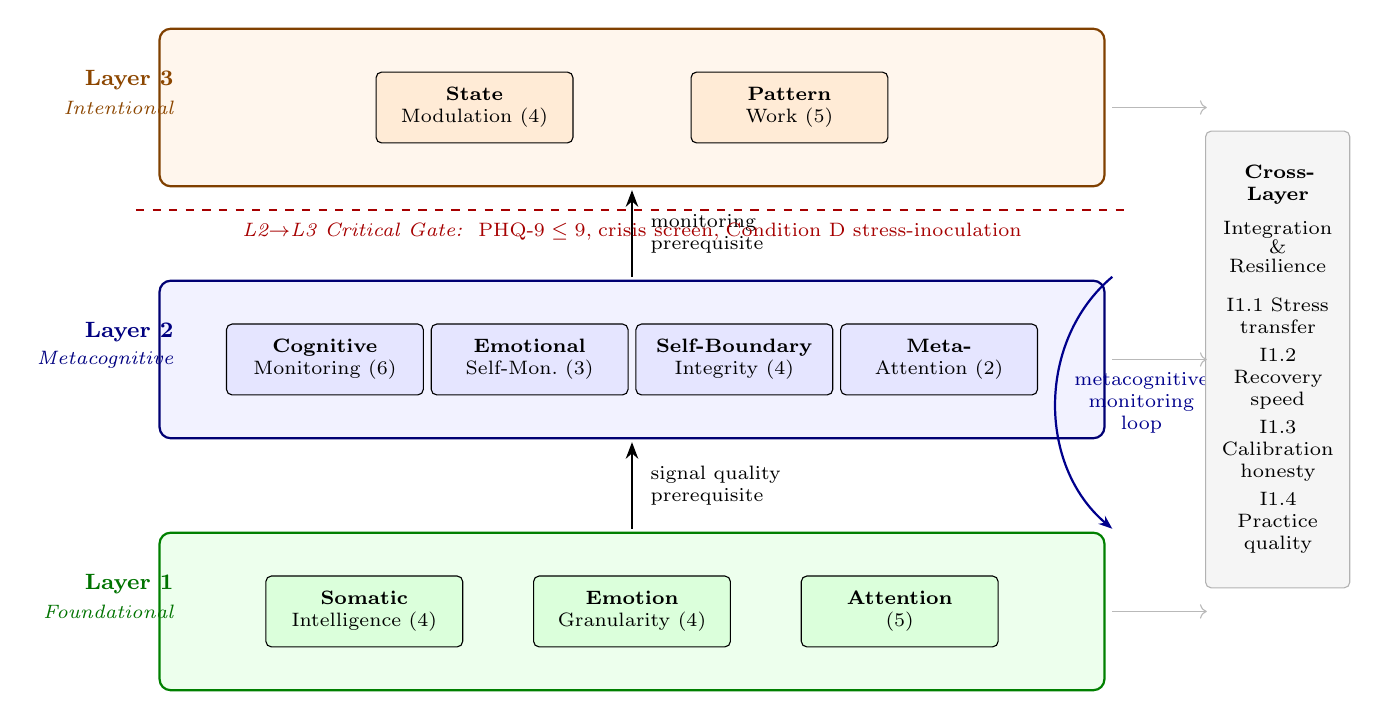
\begin{tikzpicture}[
  layerbox/.style={draw, thick, rounded corners=4pt,
    minimum width=12cm, minimum height=2cm, inner sep=5pt},
  domainbox/.style={draw, thin, rounded corners=2pt,
    minimum width=2.5cm, minimum height=0.9cm,
    align=center, font=\scriptsize, inner sep=3pt},
  depar/.style={-{Stealth[length=6pt]}, thick},
  loopar/.style={-{Stealth[length=5pt]}, thick, blue!55!black},
  gateline/.style={dashed, thick, red!65!black},
  crossbox/.style={draw=gray!60, thin, rounded corners=2pt, fill=gray!8,
    minimum width=1.7cm, align=center, font=\scriptsize, inner sep=4pt},
]

% ── Layer 1 (bottom) ─────────────────────────────────────────────────────────
\node[layerbox, fill=green!7, draw=green!50!black] (L1) at (0,0) {};
\node[font=\footnotesize\bfseries, green!45!black, anchor=east] at (-5.7, 0.35) {Layer 1};
\node[font=\scriptsize\itshape,   green!45!black, anchor=east] at (-5.7, 0.0)  {Foundational};
\node[domainbox, fill=green!14] at (-3.4, 0) {\textbf{Somatic}\\Intelligence (4)};
\node[domainbox, fill=green!14] at ( 0,   0) {\textbf{Emotion}\\Granularity (4)};
\node[domainbox, fill=green!14] at ( 3.4, 0) {\textbf{Attention}\\(5)};

% ── Layer 2 (middle) ─────────────────────────────────────────────────────────
\node[layerbox, fill=blue!5, draw=blue!45!black] (L2) at (0,3.2) {};
\node[font=\footnotesize\bfseries, blue!50!black, anchor=east] at (-5.7, 3.55) {Layer 2};
\node[font=\scriptsize\itshape,   blue!50!black, anchor=east] at (-5.7, 3.2)  {Metacognitive};
\node[domainbox, fill=blue!10] at (-3.9, 3.2) {\textbf{Cognitive}\\Monitoring (6)};
\node[domainbox, fill=blue!10] at (-1.3, 3.2) {\textbf{Emotional}\\Self-Mon.\ (3)};
\node[domainbox, fill=blue!10] at ( 1.3, 3.2) {\textbf{Self-Boundary}\\Integrity (4)};
\node[domainbox, fill=blue!10] at ( 3.9, 3.2) {\textbf{Meta-}\\Attention (2)};

% ── Layer 3 (top) ────────────────────────────────────────────────────────────
\node[layerbox, fill=orange!7, draw=orange!50!black] (L3) at (0,6.4) {};
\node[font=\footnotesize\bfseries, orange!55!black, anchor=east] at (-5.7, 6.75) {Layer 3};
\node[font=\scriptsize\itshape,   orange!55!black, anchor=east] at (-5.7, 6.4)  {Intentional};
\node[domainbox, fill=orange!16] at (-2, 6.4) {\textbf{State}\\Modulation (4)};
\node[domainbox, fill=orange!16] at ( 2, 6.4) {\textbf{Pattern}\\Work (5)};

% ── Dependency arrows ─────────────────────────────────────────────────────────
\draw[depar] (0, 1.05) -- (0, 2.15)
  node[midway, right=3pt, font=\scriptsize, align=left] {signal quality\\prerequisite};
\draw[depar] (0, 4.25) -- (0, 5.35)
  node[midway, right=3pt, font=\scriptsize, align=left] {monitoring\\prerequisite};

% ── Monitoring loop (right side) ──────────────────────────────────────────────
\draw[loopar, bend right=50]
  (6.1, 4.25) to
  node[right=3pt, font=\scriptsize, blue!55!black, align=center]
    {metacognitive\\monitoring\\loop}
  (6.1, 1.05);

% ── L2→L3 Critical Gate ───────────────────────────────────────────────────────
\draw[gateline] (-6.3, 5.1) -- (6.3, 5.1);
\node[font=\scriptsize, red!65!black, align=center] at (0, 4.82)
  {\textit{L2$\to$L3 Critical Gate:}~~PHQ-9\;$\leq9$,\;crisis screen,\;Condition~D stress-inoculation};

% ── Cross-layer skills ────────────────────────────────────────────────────────
\node[crossbox, minimum height=5.8cm, text width=1.55cm] at (8.2, 3.2)
  {\textbf{Cross-Layer}\\[4pt]Integration\\[-1pt]\&\\[-1pt]Resilience\\[6pt]
   I1.1 Stress\\transfer\\[2pt]
   I1.2 Recovery\\speed\\[2pt]
   I1.3 Calibration\\honesty\\[2pt]
   I1.4 Practice\\quality};
\draw[->, gray!55, thin] (6.1, 0.0) -- (7.3, 0.0);
\draw[->, gray!55, thin] (6.1, 3.2) -- (7.3, 3.2);
\draw[->, gray!55, thin] (6.1, 6.4) -- (7.3, 6.4);

\end{tikzpicture}
\caption{Three-layer architecture of the Mental Mastery framework. Upward arrows indicate informational prerequisites: Layer~2 metacognitive monitoring requires Layer~1 signal quality; Layer~3 pattern modification requires Layer~2 monitoring reliability. The monitoring loop (right) shows that Layer~2 observation targets Layer~1 and its own processes. The critical gate (dashed line) enforces PHQ-9, crisis, and stress-inoculation requirements before Layer~3 work is authorised. Cross-layer Integration and Resilience skills (I1.1--I1.4) apply throughout all phases.}
\label{fig:architecture}
\end{figure}

\noindent
The design principles underlying this architecture are:

\begin{enumerate}[leftmargin=2em]
\item Skills are trainable mechanisms with observable behavioural correlates, not
personality traits or fixed capacities.
\item The layer sequence is neurologically motivated: each upper layer requires the
lower layer's outputs as inputs. Layers describe \emph{functional dependencies},
not strictly sequential phases.
\item Two independent measurement tracks run throughout: Track~A (subjective and
behavioural self-report) and Track~B (physiological and performance measures).
These are explicitly \emph{not} treated as equivalent, following the finding that
neural and behavioural improvements are uncorrelated within the same measurement
window \citep{yue2023}.
\item Domain-specificity of metacognition \citep{morales2018, fleming2014} means
each of the four Layer~2 monitoring domains requires independent training and
independent assessment. High skill in one domain cannot be assumed to substitute
for another.
\item Entry is not fixed. Phase~0 assessment (Toronto Alexithymia Scale \citep{schandry1981},
Heartbeat Detection Task, FFMQ Observing Subscale) determines the individual's
starting position in Layer~1 before any training begins.
\end{enumerate}

\subsection{Taxonomic Status and Epistemic Limitations}

The 41-skill count and nine-domain structure require explicit epistemic qualification.
The taxonomy was not derived through factor analysis, latent variable modelling, or
psychometric validation of a candidate item pool. No confirmatory factor analysis
has established that the nine domains correspond to empirically separable factors,
and no item-response theory modelling has validated the skill descriptions as a
measurement instrument. The following three claims should therefore be understood
as the framework's current standing:

\begin{enumerate}[leftmargin=2em]
\item \textbf{The taxonomy is provisional.} Skill boundaries and layer assignments
were determined by convergent reading of neuroscientific mechanism and clinical
observation, not by data-driven reduction. Skills may merge, split, or be reordered
as empirical work proceeds. The 41-skill count is not a stable target; it is a
working hypothesis about the granularity at which mechanism-level distinctions
become training-relevant.

\item \textbf{The skill count is heuristic.} 41 reflects the level of analysis
at which each skill has a distinguishable neural mechanism, a distinct prerequisite
chain, and a separable assessment approach. It is not derived from, nor validated
by, any psychometric or factor-analytic procedure. Researchers treating this
taxonomy as a measurement framework should develop and validate instruments before
drawing structural inferences from the domain or skill count.

\item \textbf{Domain boundaries are functional hypotheses.} The nine domains
represent proposed clusters of mechanistically related skills. The domain-specificity
finding for metacognition \citep{morales2018, fleming2014} provides partial
neurobiological support for treating monitoring domains as distinct, but does not
validate the specific domain divisions used here. The Self-Boundary Integrity
domain (B2.1--B2.4) in particular combines skills that may prove to be dissociable
at the neural level, and whose co-clustering is currently motivated by theoretical
coherence rather than empirical convergence.
\end{enumerate}

\paragraph{Training scaffold vs.\ neural ontology.}
The taxonomy is a \emph{training design scaffold}, not a claim about neural
modularity. The 41 skills and nine domains specify what to train, in what order,
and how to assess progress; they do not claim that the brain contains 41 discrete
functional modules, or that the nine domains map cleanly onto separable neural
systems. This distinction matters for interpretation: evidence that two skills share
neural substrates, or that a domain boundary does not correspond to a confirmed
dissociation, does not falsify the training design --- it may simply mean the
scaffold is coarser or finer than the underlying neural architecture. Conversely,
discovering that B2.4 is not a trainable skill would falsify that component of the
training design while leaving the rest of the taxonomy intact. Researchers should
evaluate the taxonomy at the level at which it operates: as a structured training
programme whose components can be individually validated or refuted, not as a
proposed neural taxonomy requiring modularity evidence.

% =============================================================================
\section{Neuroscientific Foundations}
% =============================================================================

\subsection{Neuroplasticity}

Neuroplasticity is a family of related processes operating at different scales and
timescales. Synaptic plasticity following Hebb's rule \citep{hebb1949} provides the
foundational mechanism: temporally correlated pre- and post-synaptic activity
produces long-term potentiation (LTP), strengthening synaptic connections;
uncorrelated or suppressed activity produces long-term depression (LTD), weakening
them. Both are necessary: learning requires simultaneous strengthening of relevant
and suppression of irrelevant patterns.

At the structural level, cortical thickness changes are a measurable correlate of
sustained training. Right insula and somatosensory cortex thickness increases with
concurrent alexithymia reductions were demonstrated after 8-week mindfulness-based
stress reduction (MBSR) \citep{calderone2024}. Hippocampal volume increases from
the same intervention likely reflect neurogenesis in dentate gyrus, a process
enhanced by exercise and reduced by chronic glucocorticoid exposure. Functional
plasticity --- changes in how existing circuits are activated without gross structural
change --- can occur within sessions and is the mechanism underlying network
reconfiguration efficiency improvements demonstrated by \citet{yue2023}.

A critical constraint on all of the above is the behavioural relevance gate.
Plasticity does not occur through repetition alone. The cochlear implant literature
\citep{fallon2009} established that cortical reorganisation requires inputs that are
behaviourally meaningful to the organism: ``Not just any input into the wetware will
result in appropriate changes: the input must contain behaviourally important
information.'' Visual prosthetics research confirms the same principle, adding that
task variability, appropriate difficulty level, and graded feedback all modulate
plasticity durability, with positive effects persisting up to two years when
attentional neuromodulators are engaged \citep{beyeler2017}. This constraint is
operationalised in the framework as I1.4 (Practice Quality Monitoring): without it,
Layer~3 training can be high-volume and neuroplastically inert.

Individual differences in plasticity capacity are substantial and poorly
characterised. Cochlear implant outcome variance is approximately 80\% attributable
to individual ``wetware'' differences not accounted for by known factors
\citep{fallon2009}. The framework accommodates this by using individual-level
threshold demonstration rather than population-level statistics and by requiring
Phase~0 assessment to calibrate entry.

\subsection{Attention Regulation Networks}

Three large-scale brain networks govern attentional self-regulation. The
\emph{Default Mode Network} (DMN --- medial PFC, posterior cingulate cortex (PCC),
angular gyrus, hippocampus) is active during self-referential thought, autobiographical
memory, future simulation, narrative construction, and mind-wandering, which occupies
approximately 47\% of waking time in typical adults \citep{killingsworth2010}. The
PCC is the DMN's central hub; high PCC activity characterises the mind-wandering and
narrative self-generation state.

The \emph{Executive Control Network} (ECN --- dlPFC, posterior parietal cortex) is
active during goal-directed attention, working memory, and deliberate reasoning. The
ECN and DMN are typically anti-correlated at rest: activating one tends to suppress
the other. This anti-correlation is the neural architecture of voluntary attentional
control. Mindfulness training specifically increases PCC--dlPFC coupling
\citep{ganesan2025}, the neuroimaging correlate of decreased narrative self-generation
coupled with increased executive control during focused practice.

The \emph{Salience Network} (SN --- anterior insula, anterior cingulate cortex) is
the brain's relevance detector and switching system. It detects salient stimuli
(internal or external), switches between DMN and ECN modes, and processes
interoceptive signals from the body. The SN is the neural substrate of A2.2
(Dual Presence) and S1.2 (Interoceptive Accuracy). Critically, SN functional
reconfiguration efficiency improved \emph{specifically} in mindfulness practitioners
versus an active sleep hygiene control group \citep{yue2023}: less ``gear-switching
cost'' to move between internal monitoring and external task engagement.

ECN functional reconfiguration efficiency also improved specifically in the
mindfulness group across all three networks \citep{yue2023}, with the active control
group showing declines. This rest-to-task FC similarity measure is the neural basis
for M3.2 (State Shifting) as a trainable capacity with a measurable neural correlate.

\subsection{Interoception}

Interoception is the perception of the internal state of the body. The anterior
insula is the primary cortical processing centre, generating what \citeauthor{calderone2024}
describes as a moment-to-moment integrated map of the body's state. Insula cortical
thickness increases after 8-week MBSR \citep{calderone2024} provide structural
evidence that this region is trainable.

The critical qualification established by \citet{ganesan2025} is that
focused-attention breath meditation does \emph{not} reliably develop somatic
awareness: the SMS-Body subscale showed no significant group difference in a rigorous
fMRI neurofeedback RCT despite strong SMS-Mind (cognitive awareness) improvements.
Somatic Intelligence skills (S1.1--S1.4) require dedicated somatic practices ---
body scan, interoceptive tracking --- not breath-focused attention alone. This
finding directly shapes the framework's practice design: breath meditation is
insufficient for Domain~1.

The standard heartbeat detection paradigm \citep{schandry1981} is used in the
progression model as a Track~B measure of S1.2 (Interoceptive Accuracy) not because
heartbeat detection is the target skill, but because it is a research-validated
proxy for the broader interoceptive accuracy construct that correlates with emotional
awareness, body image, and anxiety regulation.

\subsection{Emotional Processing and Granularity}

The amygdala responds to salience broadly --- novel, surprising, or emotionally
significant stimuli of any valence --- rather than functioning as a single-purpose
threat detector. Emotional processing involves competition between bottom-up signals
(amygdala, insula, brainstem: fast, automatic) and top-down modulation (PFC, ACC:
slower, deliberate). This modulation requires resources: cognitive capacity,
attentional bandwidth, low baseline arousal. When PFC resources are depleted by high
cognitive load, fatigue, or acute stress, bottom-up processes dominate. This is the
neurological basis for I1.1 (Skill-Under-Load) as a cross-layer requirement.

Emotional granularity --- the precision with which one deploys emotional concepts ---
modulates regulation quality \citep{barrett2017}. People who can distinguish shame
from guilt, dread from apprehension, or tenderness from gratitude show measurably
better emotion regulation outcomes because more precise categories produce more
precisely targeted regulatory responses. E1.3 (Emotional Vocabulary Expansion) is,
at this level, structural skill training, not semantic enrichment.

Amygdala reactivity decreases after 8-week MBSR \citep{gkintoni2025}, supporting
emotional gradient detection (E1.4) at the level of automatic processing prior to
explicit labelling. MBCT's established mechanism for depression relapse prevention
relies on teaching practitioners to observe negative emotional-cognitive cascades as
events rather than facts --- a mechanism that operationally requires E1.4 to
interrupt the cascade early.

\subsection{Default Mode Network and Self-Referential Processing}

The DMN constructs the sense of a continuous, coherent self across time through
mPFC, PCC, and hippocampal integration. This has a non-trivial implication: the
narrative self --- one's beliefs about who one is, what one's history means, and
what is authentically true for oneself --- is a neurological construction rather
than a direct perception. As such, it is revisable through targeted experience.
This is the biological basis for Layer~3 existing at all.

Mind-wandering correlates with negative affect regardless of the content of the
wandering \citep{killingsworth2010}. Rumination --- DMN activity stuck in perseverative
self-referential loops --- is the pathological extreme and the mechanism underlying
depression, anxiety, and chronic stress. MBCT's evidence base across 87 studies
\citep{gkintoni2025} rests on interrupting the automatic coupling between a negative
mood and a DMN ruminative cascade. C2.6 (Narrative Monitoring) and P3.2 (Pattern
Interruption) are, at the network level, the capacity to detect and break this loop
before it completes.

B2.4 (Self-Attribution Consistency Monitoring) targets a specific source monitoring
failure mode: gradual, undetected shifts in one's own self-description arising from
sustained narrative exposure, social environment pressure, or accumulated influence
without active self-monitoring. The skill is not the preservation of a fixed
identity. Identity change, belief revision, and value development are expected,
unremarkable, and not what B2.4 addresses. The target is narrower:
\emph{metacognitive awareness of whether shifts in self-description were
consciously noticed and endorsed, or whether they accumulated below the threshold
of deliberate attention}. Operationally, this means maintaining longitudinal
self-description records and periodically comparing them against earlier records
--- not to resist change, but to detect change that occurred without active
monitoring. A practitioner who can say ``my position on X has shifted, and I
can trace when and why'' has functioning B2.4 detection. A practitioner whose
self-description has shifted substantially over six months with no conscious
record of the process has a B2.4 monitoring failure, regardless of whether the
underlying change was adaptive. The question B2.4 asks is not ``is my identity
stable?'' but ``do I know what has changed and why?''

\subsection{Metacognition}

Metacognition is cognition about cognition: monitoring, evaluating, and regulating
one's own mental processes at a level above the processes themselves. Its neural
architecture is broadly prefrontal but not uniform. The rostral anterior cingulate
cortex (rACC) and medial PFC monitor cognitive processes and generate confidence and
uncertainty signals. The inferior frontal gyrus (BA47) shows sustained and increasing
activation in advanced meditators \citep{calderone2024}, rather than habituating ---
the neural signature of deepening metacognitive engagement rather than automation.

Introspective accuracy is meaningfully skilled and partially trainable, but has hard
limits: some cognitive processes are computationally inaccessible to metacognitive
reporting even in highly trained individuals. The framework does not claim to make
all processing transparent --- it trains the accessible monitoring layer within its
genuine limits.

In predictive processing terms \citep{barrett2017}, metacognition involves monitoring
the prediction-update cycles themselves: noticing when a model is being updated,
when a prediction error is being suppressed, or when a prediction is being confused
with a percept. C2.5 (Assumption Detection) is the behavioural correlate of this:
catching when an inference is being treated as an observation.

\subsection{Neuromodulation and the Conditions for Plasticity}

Four neuromodulatory systems gate whether neural activity translates into lasting
structural change:

\emph{Dopamine} (DA), released by the VTA in response to unexpected rewards or
reward-predicting cues, opens the LTP window at synaptic sites. This is the
neurochemical basis for I1.4: engaging, meaningful practice produces more lasting
change than boring repetition, and gamification of learning contexts enhances
plasticity durability persisting up to two years by recruiting dopaminergic
reinforcement \citep{beyeler2017}.

\emph{Acetylcholine} (ACh), released by the basal forebrain during focused
attentional engagement, sharpens cortical signal-to-noise ratios and signals
``this input matters, encode it.'' Attention training (Domain~3) is partly training
the ACh-modulated gain enhancement system. Without genuine attentional focus, the
plasticity window does not open at relevant sites --- making Domain~3 a hard
biological precondition for effective Layer~2 and Layer~3 training.

\emph{Norepinephrine} (NE), released by the locus coeruleus in response to arousal
signals, follows an inverted-U relationship with cognitive performance (Yerkes-Dodson
law): optimal NE levels support sharp, engaged processing; excess NE impairs it.
Working at too difficult a performance level impedes learning through NE overshoot
\citep{beyeler2017}, constraining how stress-inoculation training must be graduated.

\emph{Brain-Derived Neurotrophic Factor} (BDNF), increased by aerobic exercise and
mindfulness practice \citep{calderone2024} and decreased by chronic glucocorticoids,
is required for many forms of LTP and supports hippocampal neurogenesis. Factors
like exercise level, sleep quality, and chronic stress are not peripheral to mental
training --- they modulate the molecular conditions under which plasticity occurs.

\subsection{Source Monitoring: The Cognitive Mechanism of Self-Boundary Integrity}

Source monitoring is the set of cognitive processes through which people attribute
the origins of their memories, beliefs, thoughts, and impulses to a particular
source \citep{johnson1993, mitchell2009}. This is the mechanism underlying the
framework's Self-Boundary Integrity domain (B2). Every B2 skill is an application
of source monitoring applied to different layers of mental content.

Memories and beliefs are reconstructed from stored feature bundles --- perceptual
detail, spatial and temporal context, semantic content, emotional tone, and records
of the cognitive operations involved in generating them. Source attribution is an
inference, not a direct read-out. Two modes operate:

\emph{Heuristic monitoring} (fast): rapid evaluation of memory quality. High
perceptual detail reads as ``probably perceived''; low contextual specificity reads
as ``probably self-generated.'' Fast, low-effort, and error-prone.

\emph{Systematic monitoring} (slow): deliberate retrieval and plausibility checking
against known facts, values, and autobiographical context. Accurate but
resource-demanding, and degraded specifically by active working memory manipulation
\citep{maniscalco2015}.

The five documented source monitoring failure modes each represent a specific
degradation pathway for source attribution robustness under competing informational inputs:

\begin{enumerate}[leftmargin=2em]
\item \textbf{Source amnesia:} Retrieved content without its source. Feels like prior
knowledge or genuine opinion. The default for information encountered without
deliberate source-encoding.
\item \textbf{Misattributed familiarity:} Repeated exposure increases processing
fluency, which heuristic monitoring misreads as evidence of authentic personal belief.
This is a primary mechanism of propaganda and large-scale social influence.
\item \textbf{Cryptomnesia:} An externally encountered idea experienced as one's own
original thought. The external encounter is forgotten; the idea returns feeling
internally generated.
\item \textbf{Incorporation of fiction as fact:} Narratively processed content is
encoded with rich perceptual and emotional detail through narrative simulation.
This richness causes heuristic monitoring to subsequently misclassify the content
as perceived rather than encountered via story.
\item \textbf{Criteria relaxation under load:} Under conditions of high arousal,
fatigue, or cognitive demand, systematic monitoring is bypassed. Heuristic monitoring
runs alone with lax criteria \citep{maniscalco2015}. This is the mechanism most
directly addressed by I1.1 (Skill-Under-Load) training.
\end{enumerate}

Two neurobiologically distinct sub-processes are involved, with different sequencing
implications \citep{simons2008}:

\emph{Context monitoring} (``was this perceived or did I generate it?'') is less
medial-PFC dependent and is more accessible to training through basic thought
observation practices. It is developed through C2.1 (Thought Observation) and E2.1
(Emotional Source Attribution).

\emph{Origin monitoring} (``did I generate this, or did another person?'') specifically
recruits medial anterior PFC (BA10) and the mentalizing network --- the circuits
that represent other people's mental states \citep{simons2008, lagioia2011}. This
is the harder, more PFC-dependent operation and the precise mechanism of B2.1
(Self-Other Signal Distinction).

Individual differences in origin monitoring capacity correlate with psychosis-proneness
(r = $-0.56$) across healthy individuals \citep{simons2008}, establishing this as a
continuous trait in the normal population, not a clinical binary. Approximately 13\%
of the healthy population has bilateral paracingulate sulcus (PCS) absence
\citep{buda2011}, associated with constitutively lower reality monitoring accuracy
\emph{and} reduced metacognitive awareness of that deficit. For these individuals,
Track~B performance assessment is the only reliable measurement channel.

Critically, this circuit is trainable: 80 hours of bottom-up perceptual precision
training in schizophrenia patients restored mPFC activation and normalised origin
monitoring accuracy, with mPFC normalisation at training completion predicting
social functioning at six-month follow-up \citep{subramaniam2012}. This constitutes
the most direct available evidence that a trainable perceptual substrate can support
higher-order boundary monitoring improvements --- a finding that motivates, but does not
confirm, the L1$\to$L2 architectural dependency claimed in this framework. The study
population (schizophrenia patients), single-site design, and absence of a healthy
adult replication cohort limit direct extrapolation; the result is treated here as
mechanistic support rather than architectural proof.

Additional design constraints from source monitoring research: \citet{moseley2018}
demonstrated that internally generated content encoded with high vividness was
subsequently more likely to be misattributed as externally perceived. Any framework
practice using mental imagery must include an explicit source-marking step during
encoding to prevent the vividness-misattribution coupling from strengthening.
\citet{bangfleming2018} established that the anterior PFC integrates confidence
signals with non-perceptual contaminants --- confidence history, current arousal,
social context --- that degrade source attribution accuracy under influence conditions.

\subsection{Source Monitoring as Primary Mechanism: Scope and Relation to Alternative Accounts}

Three other mechanisms are commonly implicated in failures of epistemic self-governance:
motivated reasoning, affective forecasting errors, and belief perseverance. Each is
well-documented. The framework's decision to build the Self-Boundary Integrity domain
around source monitoring rather than these alternatives requires justification on both
theoretical and practical grounds, and the relationship between source monitoring
and these alternatives requires explicit characterisation.

\paragraph{Basis for prioritising source monitoring.}
Three properties distinguish source monitoring from the alternatives as a primary
training target. First, it has a characterised, trainable neural substrate ---
the mPFC (BA10) origin monitoring circuit \citep{simons2008, subramaniam2012} ---
that the alternatives lack at comparable mechanistic specificity. Motivated reasoning,
belief perseverance, and affective forecasting errors are descriptions of behavioural
error \emph{patterns}; source monitoring describes the cognitive \emph{mechanism}
through which those patterns are partly instantiated during belief encoding and
retrieval. Second, source monitoring errors are, in principle, catchable in real time:
the question ``where did this belief come from, and under what conditions?'' is
an answerable question during active monitoring
\citep{johnson1993, mitchell2009}. Motivated reasoning and belief perseverance
are characteristically undetectable from the inside precisely because they operate
on evaluation and coherence-preservation after encoding has occurred.
Third, the five source monitoring failure modes provide
concrete, specifiable training targets with known activation conditions.
The alternatives do not decompose into failure modes with the same specificity.

\paragraph{Motivated reasoning: partially downstream.}
Motivated reasoning operates at the level of evidence weighting and conclusion
formation --- after a belief has been encoded and attributed. Source monitoring
failures operate upstream, at encoding: before a belief can be motivated-reasoned
about, it must have been encoded, and the source attribution assigned during that
encoding determines how revisable the belief subsequently is. A practitioner who
correctly identifies the external origin of a belief and the conditions under
which it was acquired presents a harder target for motivated reasoning than one
who holds the same belief without source records. The framework targets this
upstream step. However, motivated reasoning also has goal-directed and
identity-protective components that operate independently of source attribution
accuracy --- a practitioner may correctly identify a belief's external origin and
still be motivated to preserve it. The framework addresses this residual through
I1.3 (Calibration Honesty), which specifically trains tolerance of uncertainty
and resistance to motivated misreporting. But I1.3 is not a motivated reasoning
intervention; it is a calibration practice. The framework does not claim to
eliminate motivated reasoning.

\paragraph{Affective forecasting errors: largely independent.}
Affective forecasting errors --- systematic mispredictions of future emotional
states --- stem from simulation failures: immune neglect, focalism, and
mispredicted hedonic adaptation rates. These are errors in prospective emotional
simulation, not in the attribution of current belief origins. Source monitoring
training does not directly address them. Emotion granularity development (E1.2)
and interoceptive accuracy (S1.2) improve current-state signal quality, which
may reduce the systematic biases that feed prospective simulation, but this is
a secondary effect rather than a design target. Researchers should not interpret
the framework's emotional processing components as extending to affective
forecasting accuracy. This is a genuine gap: practitioners who complete the full
progression may still show standard affective forecasting error magnitudes.

\paragraph{Belief perseverance: partially downstream.}
Belief perseverance --- the tendency for beliefs to persist after their
evidential basis has been discredited --- is partially downstream of source
monitoring. If a practitioner can attribute the origin and evidential conditions
of a belief, they are better positioned to update it when those conditions
change. B2.3 (Value Anchoring) and the longitudinal documentation component
of B2.4 address this in part by maintaining a reference structure against which
belief change can be evaluated. However, belief perseverance also has
coherence-protection and identity-continuity components that are partially
independent of source attribution accuracy. The framework's coverage here is
incomplete --- and deliberately disclosed as such: B2.4 has been classified as
a hypothesised extension rather than a confirmed trainable skill (Section~10.3),
precisely because the identity-stability mechanism is not yet operationalised
or empirically validated.

\paragraph{Summary position.}
The framework treats motivated reasoning and belief perseverance as
\emph{partially downstream} of source monitoring: source monitoring training
reduces their material supply (unattributed beliefs available for motivated
processing) but does not address their motivational or coherence-preserving
components. The framework treats affective forecasting errors as
\emph{largely independent}: a different class of error, not covered by the
current design. Stating this explicitly is not a weakness; it is the boundary
that makes the framework's central hypothesis testable.

\subsection{Two-Tier Metacognitive Architecture and Domain-Specificity}

Three converging studies establish that metacognition is not a unified capacity
\citep{morales2018, shekhar2018, fleming2014}:

\emph{Level~1 (domain-general)}: Encoded in the dACC/insula/cingulo-opercular
network. Generates a generic confidence and accuracy signal that partially predicts
performance across all cognitive domains. A classifier trained on one domain's
patterns predicts confidence in a different domain. This layer is the neural
substrate of I1.4 (Practice Quality Monitoring) and partially transfers across
domains.

\emph{Level~2 (domain-specific)}: Encoded in the aPFC/right rostrolateral PFC
(BA10). Carries domain-specific metacognitive accuracy representations that do
\emph{not} generalise. Individual metacognitive scores for perception and memory
are uncorrelated ($r = -0.076$) \citep{morales2018}. Anterior PFC lesions selectively
impair perceptual metacognition while leaving memory metacognition intact ---
causal, not merely correlational, evidence for domain-specificity \citep{fleming2014}.

A large-sample fMRI study ($n = 308$) found that higher metacognitive accuracy
correlates with \emph{less} aPFC activation \citep{molenberghs2016}: skilled
metacognition is neurally efficient, not effortful. Early monitoring is effortful;
competence feels like the same accuracy with less cost. The same study found that
acknowledged uncertainty activates OFC/insula (associated with negative affect),
while false confidence activates bilateral striatum (dopaminergic reward circuits).
This creates a motivated bias toward false certainty that calibration training
must address through explicit tolerance of acknowledged not-knowing --- an emotional
regulation requirement embedded within metacognitive skill development, and a reason
why E1 (Emotion Granularity) is a prerequisite for reliable Layer~2 self-monitoring.

The critical practical implication: somatic monitoring skill (S1 domain) does not
substitute for emotional monitoring skill (E2 domain), which does not substitute for
cognitive monitoring (C2 domain), which does not substitute for self-boundary
monitoring (B2 domain). Each requires its own dedicated training and independent
assessment.

\subsection*{Landmark Convergent Findings}
\addcontentsline{toc}{subsection}{Landmark Convergent Findings}

Table~\ref{tab:convergence_condensed} summarises the eight most consequential
convergent findings for framework design. Each finding simultaneously constrains
what the framework claims and motivates a specific structural choice. The full
cross-paper convergence table appears in Section~11.

\begin{table}[htbp]
\centering
\caption{Landmark Convergent Findings and Their Structural Implications
         (condensed; full detail in Table~\ref{tab:convergence})}
\label{tab:convergence_condensed}
\small
\begin{tabular}{p{4.5cm}p{2.8cm}p{5.2cm}}
\toprule
\textbf{Finding} & \textbf{Key Sources} & \textbf{Structural Implication} \\
\midrule
Insula/SN is the trainable interoceptive substrate; breath meditation insufficient for somatic awareness &
  \citet{calderone2024, yue2023} &
  Dedicated somatic practices required in Layer~1 \\[4pt]
ECN--DMN dynamics are the substrate of attentional self-regulation &
  \citet{ganesan2025, yue2023} &
  Domain~3 attention training is a biological precondition for Layer~2 \\[4pt]
PFC-dependent regulation fails under acute physiological stress &
  \citet{raio2013} &
  Skill assessment under load is required; calm-only evaluation is insufficient \\[4pt]
Source monitoring failure modes are the mechanism of influence vulnerability &
  \citet{johnson1993, mitchell2009, simons2008} &
  B2 domain structured around five specific, named failure modes \\[4pt]
Metacognitive accuracy is domain-specific; does not transfer across domains &
  \citet{morales2018, fleming2014} &
  Each monitoring domain requires independent training and assessment \\[4pt]
mPFC (BA10) origin monitoring circuit is trainable via bottom-up perceptual training &
  \citet{subramaniam2012} &
  Layer~1 perceptual substrate enables Layer~2 boundary monitoring \\[4pt]
Practice ratio predicts resilience outcomes; minimum effective dose $\approx$11 min/day &
  \citet{jha2015, jha2016, jha2017, jha2020} &
  Quality and practice ratio are operationally critical variables \\[4pt]
Neural and behavioural change are decoupled within the same measurement window &
  \citet{yue2023} &
  Two independent measurement tracks are required throughout \\
\bottomrule
\end{tabular}
\end{table}

% =============================================================================
\subsection{Translational Assumptions}
% =============================================================================

The framework extrapolates from four categories of existing research to a target
context --- healthy adults, long-term self-directed training --- that none of
those categories directly studies. The extrapolations are listed explicitly here
so that readers can evaluate each step independently.

\begin{enumerate}[leftmargin=2em]

\item \textbf{From clinical to healthy populations.} The most direct evidence
for mPFC origin-monitoring trainability comes from schizophrenia patients
\citep{subramaniam2012}. Clinical populations undergoing targeted remediation
may show training effects substantially different in magnitude, mechanism, or
trajectory from those achievable in unimpaired individuals. The framework
assumes that if the circuit is trainable when significantly compromised, a less
intensive training effect is available to those with intact but undeveloped
function. This assumption is plausible but untested.

\item \textbf{From short-term RCTs to long-term training.} The mindfulness and
attentional training literature primarily measures outcomes at 8--12 weeks
\citep{jha2015, jha2016, jha2017, jha2020, ganesan2025}. The framework's
full progression is structured across 24+ weeks, with Layer~3 outcomes
hypothesised to require months to years. Whether effects observed in short-term
RCTs extrapolate to, accumulate across, or require fundamentally different
mechanisms at longer timescales is not established.

\item \textbf{From resting-state FC to active-monitoring function.} Several
mechanistic claims rest on resting-state functional connectivity studies
\citep{yue2023, grani2025}. Resting-state FC is a valid neural marker but
is not equivalent to functional capacity during demanding cognitive tasks.
The framework's monitoring architecture (Section~5) is described at the
functional level; the resting-state evidence provides mechanistic plausibility,
not direct functional validation.

\item \textbf{From structural neuroimaging to training-induced change.}
Structural differences between experienced practitioners and novices
\citep{calderone2024} establish that long-term practice correlates with
structural brain change. Cross-sectional comparisons cannot establish that the
observed structural differences were caused by training rather than reflecting
pre-existing individual differences. Longitudinal within-subject designs showing
structural change as a function of practice are required for causal inference.

\end{enumerate}

None of these translational steps is unreasonable; each is supported by at
least partial evidence. But the framework's overall claim --- that a specific
long-term training programme in healthy adults produces measurable improvement
in source attribution robustness under real-world informational conditions ---
requires validation across all four steps simultaneously. No existing study
addresses this composite claim.

% =============================================================================
\section{The Three-Layer Sequence: Neurological Justification}
% =============================================================================

\subsection{Layer 1 to Layer 2 Dependency}

Layer~1 builds the sensors: interoceptive accuracy (insula, salience network),
emotional signal quality (amygdala-to-insula mapping, emotional granularity), and
attentional stability (ECN--DMN anti-correlation). Layer~2 builds the monitoring
system: prefrontal metacognition observing the outputs of Layer~1 processes.

The key dependency is that if the sensors are noisy or absent, metacognition has
nothing reliable to observe. A person with significant alexithymia attempting C2.1
(Thought Observation) will be working with heavily filtered, inaccurate input.
Their ``observation'' of thoughts will be partially observation and partially
construction, and I1.3 (Calibration Honesty) will be correspondingly degraded.

The Phase~0 screening for alexithymia (TAS-20) and interoceptive accuracy (Heartbeat
Detection Task \citep{schandry1981}) implements this dependency: before training the
monitoring system, verify that the signals it will monitor are sufficiently clear.

Acetylcholine provides a second dependency: Domain~3 attention training is partly
training the ACh-modulated gain enhancement system. Without sustained, directed
attention on internal processes, metacognitive signals are too noisy to be reliably
read. Domain~3 is not a soft prerequisite --- it is a hard biological precondition.

\subsection{Layer 2 to Layer 3 Dependency}

Layer~3 involves deliberate modification of cognitive and emotional patterns.
At the neural level, this means intentionally targeting circuits for LTP or LTD
through directed, behaviourally relevant practice. The critical point: you cannot
reliably modify a circuit you cannot accurately perceive. If Layer~2 monitoring
is unreliable, Layer~3 practice will produce change, but the practitioner will
be unable to verify whether the target pattern is actually changing, whether an
adjacent unintended pattern is also being modified, or whether the modification
is producing a harmful side effect.

The history of psychological intervention contains numerous examples of techniques
that produce changes --- but not the changes intended, or with unmonitored side
effects. The difference between systematic skill training and potentially harmful
self-modification is whether the monitoring system (Layer~2) is reliably operational
before modification work begins. This is the mechanism behind the framework's safety
warning at Layer~3: ``Operating here without solid Layer~2 capability means modifying
patterns you cannot accurately perceive. This is the layer where harm becomes
possible.''

\subsection{The L2-to-L3 Gate as a Safety Requirement}

The framework's L2$\to$L3 gate --- requiring demonstration of skill under load
conditions including mild physiological arousal, a PHQ-9 score below the clinical
moderate threshold, and absence of active crisis indicators --- is not a curriculum
checkpoint. It is a functional safety requirement grounded in: (1) the stress-transfer
problem \citep{raio2013} requiring that skills be tested under the conditions in which
they must operate; (2) the known PFC vulnerability to glucocorticoid-mediated
impairment during depressive episodes \citep{gkintoni2025}; and (3) the pattern
modification risk identified above. The gate cannot be waived without removing
these safety functions.

\subsection{Why the Sequence Is Necessary: Anticipated Objections}

The composite architecture claim invites four specific challenges. Each has a
direct answer grounded in the mechanisms already established.

\paragraph{Why assume additive or synergistic effects?}
The framework makes no additive or synergistic claim. The three layers are
\emph{constitutive} components of a single target capacity, not separate
capacities whose effects combine. Source attribution robustness under load
requires: (a)~accurate interoceptive and emotional signals to monitor,
(b)~a monitoring system calibrated to those signals, and (c)~the ability
to sustain that monitoring under physiological and cognitive stress. No
component alone produces the outcome; all three are necessary conditions.
A monitoring system with no reliable input cannot monitor. A practitioner
with reliable signals but no monitoring system cannot observe them. A
practitioner with both but without stress-transfer training fails at the
moment monitoring is most needed. The question is not whether the components
add --- it is whether each is necessary. The existing evidence says yes
for each individually; the composite test is the outstanding empirical question.

\paragraph{Why this specific sequencing?}
Sequencing is constrained by informational dependency, not design preference.
The critical mechanism: Layer~2 monitoring detection thresholds are set
during training. A monitoring system trained on Layer~1 signals of insufficient
quality is calibrated to poor-quality input --- its thresholds encode the noise
level it encountered during development. Improving the sensors afterwards does
not automatically recalibrate the monitor; the monitor's sensitivity was set
by its training environment. This means the input substrate must reach minimum
fidelity before monitoring training begins, not as a soft scheduling preference
but as a condition for the monitoring system to develop correct sensitivity.
The Phase~0 screening for alexithymia and interoceptive accuracy implements
this directly: it verifies the substrate quality before monitoring training
is authorised.

\paragraph{Why not parallel training?}
Within-layer parallelism is explicitly supported and used: somatic accuracy,
emotional granularity, and attentional stability develop simultaneously within
Layer~1. Between-layer parallelism is the claim this objection targets. The
threshold-calibration argument above is a mechanistic hypothesis, not an
established finding: it predicts that parallel Layer~1 and Layer~2 training
will produce lower source attribution accuracy at the Layer~2 gate than
sequential training, because the monitoring system's sensitivity thresholds
will have been set against a moving and initially degraded input signal rather
than a stable, mature one. The sequencing architecture therefore makes a
specific testable prediction: practitioners randomised to simultaneous
Layer~1/Layer~2 training will show lower origin-monitoring accuracy and higher
calibration error at the Layer~2 exit assessment than practitioners randomised
to sequential training, even when total training hours are equated. This
prediction is directly testable by the randomised design described in the
Potential Falsification Pathways section. The claim is architectural --- not
yet empirical.

\paragraph{Why not a reduced architecture?}
A reduced architecture may be sufficient; we do not know, because no
component-ablation study has compared full vs.\ layer-skipping protocols.
The framework specifies the complete architecture because it is internally
consistent with the mechanisms --- every component addresses a documented
failure mode that the others do not cover. Somatic and emotional Layer~1
skills are not interchangeable with attentional Layer~1 skills; each removes
a distinct source of monitoring error. If a reduced architecture reaches the
same outcome at lower training cost, that would be an important and useful
finding --- not a falsification of the framework, but a specification of its
minimum viable form. This comparison is listed explicitly as a research
priority in the Potential Falsification Pathways section (Section~10).

% =============================================================================
\section{Probabilistic Monitoring Architecture: Channels, Mechanisms, and Known Failure Modes}
% =============================================================================

\subsection{Channels of Subconscious Influence}

Any technique capable of subconscious influence must operate through a limited set
of channels: (1) bottom-up sensory input generating an emotional response before
cortical awareness; (2) source monitoring failure --- externally introduced content
misattributed as self-generated; (3) narrative priming that makes certain thoughts
feel natural, true, or self-generated; (4) emotional contagion shifting affective
state before attribution occurs; (5) arousal manipulation that degrades PFC function;
and (6) unmonitored self-description drift through sustained exposure to narratives
or social environments without active metacognitive tracking of self-concept change.

Emotional contagion warrants specific attention as a framework target. It operates
through multiple simultaneous mechanisms: facial mimicry activating corresponding
muscle groups and generating associated interoceptive signals; limbic resonance
evidenced in inter-brain theta and beta coherence during social interaction
\citep{chen2022}; and parasocial/media-mediated contagion exploiting narrative
simulation mechanisms. E2.2 (Emotional Contagion Awareness) is the first-line
detection skill for this channel, requiring the prerequisite E1.4 (Emotional
Gradient Detection) to catch the early signal.

\subsection{Detection and Resistance by Channel}

\begin{longtable}{p{3.5cm}p{4.5cm}p{5cm}}
\toprule
\textbf{Influence Channel} & \textbf{Detection Mechanism} & \textbf{Resistance Mechanism} \\
\midrule
\endhead
Bottom-up emotional signal &
  E1.4 gradient detection + E2.1 source attribution &
  B2.1 self-other distinction; M3.4 response modulation before full capture \\[4pt]
Source monitoring failure &
  B2.1 origin monitoring + C2.5 assumption detection + B2.2 incongruence vs.\ values &
  Systematic source-checking habit; values document as external anchor (B2.3) \\[4pt]
Narrative priming &
  C2.6 narrative monitoring + C2.5 assumption detection &
  B2.2 incongruence detection; P3.2 pattern interruption breaks the chain \\[4pt]
Emotional contagion &
  E2.2 contagion awareness + S1.3 baseline deviation &
  A2.2 dual presence during exposure; B2.3 value anchoring \\[4pt]
Arousal manipulation &
  S1.4 arousal detection + C2.4 cognitive load sensing &
  M3.1 voluntary relaxation (parasympathetic, PFC-independent); I1.2 recovery speed \\[4pt]
Unmonitored self-description drift &
  B2.4 (self-description drift detection) + I1.3 calibration honesty &
  Longitudinal self-description records; periodic comparison detects unendorsed change \\
\bottomrule
\caption{Detection and Resistance Mechanisms by Influence Channel}
\label{tab:firewall}
\end{longtable}

\subsection{The Stress-Transfer Problem}

\citet{raio2013} demonstrated experimentally that cognitive emotion regulation
strategies --- reappraisal and acceptance, both taught and practised under calm
conditions --- produced \emph{zero} reduction in conditioned fear responses when
acute physiological stress was induced before application. The stressed group's
fear responses were statistically equivalent to pre-training acquisition levels
despite having received identical training to the non-stressed group.

The mechanism is noradrenergic, not motivational or effort-related. Acute sympathetic
arousal rapidly degrades dorsolateral PFC function through NE overshoot. The same
PFC systems that support deliberate reappraisal, perspective-taking, pattern
interruption, and all Layer~2 and Layer~3 skills that rely on cognitive override
are impaired. This is a state-dependent neurobiological constraint, not a training
intensity problem.

The practical implications are severe: Layer~2 and Layer~3 skills assessed only
under calm conditions are measuring a capability that is \emph{less relevant} than
real-world deployment capability. The conditions under which the framework's
monitoring system must operate --- arousal, social pressure, emotional activation --- are
precisely the conditions under which PFC-dependent strategies are most impaired.

\textbf{Mitigations (not eliminations):}
\begin{itemize}[leftmargin=2em]
\item Stress-inoculation training is required in Phases~7--8: skills must be
practised immediately after mild physiological arousal induction (vigorous exercise,
cold exposure, mild social challenge), not only from calm baseline.
\item The L2$\to$L3 gate specifically requires demonstration of skill under
physiological arousal condition (Condition~D in the B8 Load-Condition Assessment),
not only under cognitive or emotional load at rest.
\item Somatic and parasympathetic regulation (M3.1 --- operating downstream of PFC)
are less vulnerable than cognitive override approaches. Layer~1 somatic grounding
is the fastest available stress-response that does not depend on PFC resources.
\item Skills trained toward automaticity through sustained Layer~3 practice reduce
PFC cost per deployment, making them more stress-resistant. But automaticity must
be \emph{tested} under arousal, not assumed from calm-condition performance.
\end{itemize}

\subsection{Additional Structural Limits}

Extreme arousal (acute fear, rage) bypasses PFC entirely --- no trained skill
survives amygdala hijack intact. The framework mitigates this through proactive
arousal detection and regulation (M3.3) before conditions deteriorate, not recovery
during them.

Metacognitive monitoring is suppressed during active working memory manipulation
\citep{maniscalco2015}. Ruminative, planning, and worry states involve exactly this
kind of manipulation: the states in which practitioners most want to self-monitor
are neurobiologically the states in which self-monitoring is least reliable. Layer~1
somatic grounding and attentional stabilisation must precede metacognitive attempts
when the individual is in an active-manipulation cognitive state. This is documented
as a named failure mode in the framework's progression model, not left as an
implicit limitation.

Sufficiently subtle influence may not produce detectable deviation: if influence is
calibrated to stay within the practitioner's noise threshold, B2.1 will not fire.
Detection is probabilistic, not absolute.

Trained monitoring skills require ongoing maintenance. Skills that are not practised
decay, with structural changes (cortical thickness, connectivity) persisting longer
than functional habits. This makes Phase~8 (ongoing 12-week checkpoints) a design
necessity, not a rounding off of the programme.

% =============================================================================
\section{Critical Design Constraints}
% =============================================================================

\subsection{Domain-Specificity of Metacognition}

The domain-specific layer of metacognition (aPFC, BA10) carries domain-specific
representations that do not generalise \citep{morales2018, fleming2014}. A
practitioner with excellent Cognitive Process Monitoring (C2 domain) cannot be
assumed to have equivalent Emotional Self-Monitoring (E2), Self-Boundary Integrity
(B2), or Somatic monitoring (S1). Each domain requires its own dedicated training
and must be independently assessed. This directly constrains the framework's
assessment design: gate criteria in each domain are assessed independently, and
discrepancies between domains are surfaced explicitly rather than averaged away.

\subsection{Metacognitive Unavailability Under Working Memory Load}

Active working memory manipulation --- as distinct from mere maintenance ---
specifically degrades metacognitive sensitivity \citep{maniscalco2015}. Ruminative,
planning, and worry states involve this manipulation. The framework's response is:
(1) name this explicitly as a failure mode in practitioner training, so that
practitioners know when they are attempting monitoring in a state that prevents
reliable monitoring; (2) design Layer~1 grounding practices as the initial response
to this state, restoring preconditions before Layer~2 monitoring is attempted.

\subsection{Behavioural Relevance as a Plasticity Gate}

Plasticity requires behaviourally meaningful input \citep{fallon2009, beyeler2017}.
``Not just any input into the wetware will result in appropriate changes.''
Quantity of practice without quality does not produce structural change. The framework
implements I1.4 (Practice Quality Monitoring) as a required cross-layer skill
introduced at the Layer~3 entry point, with specific quality conditions: behavioural
relevance, appropriate challenge level (not too easy, not overwhelming), contextual
variety, and intentional engagement. Practitioners without I1.4 can generate
high-volume, neuroplastically inert sessions.

Four independent studies by \citet{jha2015}, \citet{jha2016}, \citet{jha2017}, and
\citet{jha2020} converge on identifying a minimum effective dose of approximately
11 minutes per day of formal practice and, critically, that practice \emph{ratio}
(proportion of time practised vs.\ time given) predicts cognitive resilience
outcomes more strongly than total dose. Below threshold, decline is the default;
the framework trains against decline, not only for enhancement.

\subsection{The BCT Inversion}

The Breath Counting Task (BCT) accuracy declined in the group showing the strongest
neural and subjective improvement in \citet{ganesan2025}. The likely mechanism:
the trained group developed genuine decentering --- awareness of the act of counting
as a mental process --- which interfered with the mechanical execution of counting.
This is not attentional failure; it is a shift from automatic execution to
meta-aware execution. The BCT and related standard neuropsychological attention tests
should not be used as primary skill progress markers; multiple reviews report
inconsistent improvement after 8-week MBIs \citep{calderone2024, gkintoni2025}.
Neural efficiency measures (ECN reconfiguration, PCC--dlPFC coupling) or
ecologically valid tasks are preferred.

% =============================================================================
\section{Training Design Principles}
% =============================================================================

The framework's 35 named practices are organised across a Phase~0--8 progression
with weekly schedules and phase exit assessment checklists. Core design principles
derived from the evidence review:

\begin{enumerate}[leftmargin=2em]
\item \textbf{Dedicated somatic practices are required.} Breath-focused meditation
is insufficient for Domain~1 skills \citep{ganesan2025}. Body scan and interoceptive
tracking must be explicitly scheduled, not assumed to be covered by seated meditation.

\item \textbf{Load-condition training is required.} Skills trained only in calm,
low-distraction conditions will not transfer to the conditions in which they are
needed \citep{raio2013, beyeler2017}. Each domain's skills must be practised under
conditions that approximate deployment conditions.

\item \textbf{Context monitoring before origin monitoring.} B2.1 (origin monitoring)
is trained after C2.1 (thought observation) and E2.1 (emotional source attribution),
following the neurobiologically supported sequencing: context monitoring first
(less medial-PFC dependent), then origin monitoring \citep{simons2008}.

\item \textbf{Targeted pattern interruption requires targeted training.} Standard
mindfulness does not reduce impulsivity in naive practitioners \citep{calderone2024,
gkintoni2025}. P3.2 (Pattern Interruption) requires deliberate interruption
training aimed at the specific habit chains identified through topology mapping
(P3.4), not general mindfulness practice.

\item \textbf{Source-marking is required in all visualisation practices.}
Any practice using mental imagery must include an explicit ``this is self-generated
content'' step during encoding, to prevent the vividness-misattribution coupling
from strengthening \citep{moseley2018}.

\item \textbf{Two independent tracks must be maintained throughout.} Track~A
(self-report) and Track~B (physiological/performance measures) are not substitutes.
Brain and behavioural changes are uncorrelated within the same measurement window
\citep{yue2023}, and approximately 13\% of the population has a structural deficit
that makes Track~A systematically biased \citep{buda2011}. Both tracks are required.

\item \textbf{The minimum effective dose is approximately 11 min/day} of formal
practice, with the critical variable being practice \emph{ratio}, not total hours
\citep{jha2015, jha2016, jha2017, jha2020}. Quality, not quantity, determines
plasticity outcomes \citep{fallon2009}.
\end{enumerate}

% =============================================================================
\section{Assessment Framework}
% =============================================================================

The assessment framework comprises six validated instruments (Toronto Alexithymia
Scale TAS-20; FFMQ Observing Subscale; SMS-Mind; PHQ-9; DASS-21; Rumination Response
Scale) and eleven custom protocols (B1--B11, covering somatic baseline, heartbeat
detection, arousal calibration, vocabulary audit, attention sustaining, direction and
discrimination, distraction resistance, meta-attention probe, dual presence
performance, load-condition matrix, and calibration honesty check). Nineteen journal
templates standardise longitudinal self-report. Phase gate checklists for all nine
transitions formalize threshold requirements.

The B8 Load-Condition Assessment warrants specific notation: skills are rated under
five conditions (rested baseline plus four load conditions --- cognitive, emotional,
social, and physiological arousal). Condition~D (physiological arousal, induced
immediately after vigorous exercise or cold exposure) is required for the L2$\to$L3
gate, implementing the stress-transfer problem mitigation directly in the assessment
design rather than leaving it to practitioner discretion. Retention is scored as
mean skill rating across all four load conditions as a percentage of rested baseline.

\paragraph{Physiological verification and compliance limits.}
Stress induction for Condition~D is practitioner-executed: the app cannot induce
exercise or cold exposure. HR verification is available when a Bluetooth LE heart
rate monitor is paired; in that configuration, the app gates assessment start
behind a verified HR threshold, providing objective confirmation that sympathetic
activation preceded skill testing. When no HR monitor is connected, HR verification
is not performed and Condition~D reflects protocol adherence only --- the
practitioner's self-report that the prescribed stress protocol was completed ---
not confirmed sympathetic activation. This is a meaningful distinction.
A practitioner who completes the prescribed physical protocol without achieving
target HR elevation (due to fitness level, timing, or protocol deviation) will
produce a Condition~D score that does not validly index stress-transfer capacity.
Researchers using the B8 assessment in formal studies should treat verified
Condition~D scores (HR-gated) and unverified scores as separate data classes,
and report the proportion of verified administrations. In self-directed use,
this limitation is disclosed to practitioners in the app and noted in the
assessment output.

Criterion types are distinguished in the gate system: \emph{auto} criteria are
computed directly from assessment results; \emph{semi-auto} criteria are computationally
evaluable but require explicit practitioner acknowledgment (used for crisis indicators);
\emph{manual} criteria require practitioner attestation from journal-based,
longitudinal, or behavioural evidence. Gate~7 (L2$\to$L3) contains PHQ-9 and
crisis-indicator criteria flagged as \emph{hard blocks} (the gate cannot pass if
these criteria fail, regardless of other scores).

\subsection{Phase Validation Targets}

Table~\ref{tab:phase_validation} specifies the minimum exit criteria for each
of the nine phase transitions. Track~A targets are subjective and behavioural;
Track~B targets are physiological and performance-based. Both tracks must meet
their respective thresholds unless documented individual-difference factors
justify clinician-supervised adjustment. B-codes refer to the custom assessment
protocols described in the full progression model; threshold values are as
specified therein and summarised here for cross-reference.

\begin{longtable}{p{1.1cm} p{2.3cm} p{4.9cm} p{4.9cm}}
\caption{Phase Exit Validation Targets by Measurement Track}
\label{tab:phase_validation} \\
\toprule
\textbf{Phase} & \textbf{Domain Focus} & \textbf{Track A Exit Target} & \textbf{Track B Exit Target} \\
\midrule
\endfirsthead
\multicolumn{4}{l}{\small\textit{(Table~\ref{tab:phase_validation} continued)}} \\
\toprule
\textbf{Phase} & \textbf{Domain Focus} & \textbf{Track A Exit Target} & \textbf{Track B Exit Target} \\
\midrule
\endhead
\bottomrule
\endfoot

0$\to$1 &
  Entry screening &
  TAS-20, FFMQ Observing, and SMS-Mind administered; entry track (standard / extended / priority) assigned per instrument scores &
  B1 somatic detection baseline recorded; Heartbeat Detection Task completed; 0--10 arousal scale calibrated \\[4pt]

1$\to$2 &
  L1: Somatic and attentional foundation &
  Somatic event log maintained $\geq$3 weeks; S1.4 arousal self-ratings within $\pm$2.0 of B3 check; $\geq$3 emotion categories reliably named &
  B1 somatic detection $\geq$60\%; B5a sustained attention $\geq$10~min without reset; B3 arousal calibration error $\leq$2.0 (0--10 scale) \\[4pt]

2$\to$3 &
  L1: Emotional literacy and attentional depth &
  TAS-20 $\leq$60 or meaningful reduction from baseline; FFMQ Observing $\geq$30; emotion-sensation mapping $\geq$80\% non-neutral &
  B4 vocabulary audit $\geq$40 distinct descriptors; B5b distraction resistance criteria met; B3 arousal error $\leq$2.0 sustained \\[4pt]

3$\to$4 &
  L1$\to$L2 bridge &
  C2.1 thought observation consistent $\geq$3 weeks (journal evidence); B2.1 source-checking entry behaviour documented &
  B6 meta-attention probe pass; B11 calibration matrix baseline complete; A2.1 auto-evaluated from B6 \\[4pt]

4$\to$5 &
  L2: Metacognitive core &
  SMS-Mind $\geq$35; C2.4 cognitive load sensing self-ratings calibrated against B8 Condition~A baseline &
  B8 Conditions A/B/C $\geq$70\% skill retention vs.\ rested baseline; B9 meta-attention probe pass \\[4pt]

5$\to$6 &
  L2: Self-boundary and dual presence &
  B2.1--B2.3 source-monitoring skills consistent $\geq$4 weeks; I1.3 calibration honesty log $\geq$6 weeks without inflation; A2.2 dual presence under moderate load documented &
  B8 Conditions A/B/C $\geq$70\% retention; B10 dual presence performance pass; B11 $\geq$2 load conditions calibrated \\[4pt]

6$\to$7 &
  \textbf{Critical L2$\to$L3 safety screen} &
  PHQ-9 $\leq$9 (\emph{hard block}); active crisis indicators absent (\emph{hard block}); FFMQ Observing $\geq$38; RRS $\leq$35; B2.4 longitudinal self-attribution records documented $\geq$12 weeks &
  B8 all four conditions (A/B/C/D) $\geq$70\% retention; Condition~D (physiological arousal) mandatory; B11 $\geq$3 load conditions; M3.4 resting HR baseline and somatic signature recorded \\[4pt]

7$\to$8 &
  L3: State modulation exit &
  M3.1--M3.3 voluntary parasympathetic activation documented $\geq$4 weeks; I1.2 emotional recovery speed within individual target window &
  B8 Condition~D maintained $\geq$70\% under physiological load; HR delta recovery documented within target \\[4pt]

8, 12-wk &
  L3: Pattern work checkpoint (ongoing) &
  I1.1 stress-transfer: B8 stress-condition performance $\geq$70\% of rested baseline across all six target skills; I1.4 practice quality monitoring consistent &
  Full 5-condition B8 matrix updated; B11 calibration matrix updated across all conditions \\

\end{longtable}

\subsection{Implementation Status}

The Mental Mastery framework is presented as an operational specification
intended for software implementation. The three-layer structure, domain
separation, phase progression, and gate logic are defined at a level of
precision suitable for direct encoding in an application environment. The
framework is being implemented as an Android mobile application (Flutter,
offline-first, local database) whose architectural role is to impose structural
rigidity on the progression --- preventing the protocol drift that occurs in
self-directed use when practitioners manage gate criteria informally.

The implementation will:

\begin{itemize}[leftmargin=2em]
\item \textbf{Enforce phase gates programmatically.} Gate criteria are encoded
as static framework content (auto, semi-auto, and manual criterion types).
Progression is blocked without demonstrated criteria satisfaction. The
L2$\to$L3 hard-block logic (PHQ-9 $\geq10$, active crisis indicators) is
enforced in code --- the gate cannot pass regardless of other scores, and this
constraint cannot be overridden by the practitioner.

\item \textbf{Maintain dual measurement tracks.} Track~A (subjective and
behavioural) and Track~B (physiological and performance) are recorded
independently throughout. Where a Bluetooth LE heart rate monitor is paired,
HR data is integrated directly into Track~B records. Track A/B discrepancies
are surfaced explicitly at gate evaluations rather than averaged away.

\item \textbf{Require demonstration of skill under load before authorising
Layer~3 work.} Condition~D (physiological arousal) data must be present and
meet threshold before the L2$\to$L3 gate can pass. As described in the
preceding section, verified Condition~D scores (HR-gated) and unverified scores
are distinguished in the record.

\item \textbf{Log anonymised aggregate metrics to support future empirical
evaluation.} With practitioner opt-in (not at installation; after Phase~0),
anonymised aggregate data --- time-to-gate, pass/fail distributions, Track~A/B
convergence patterns, Condition~D retention under load --- is retained for
population-level analysis. No journal content, audio, transcripts, or
self-assessment text is ever included. Extraction is opt-in and purpose-limited.
\end{itemize}

The implementation is intended as an executable test of the architectural
hypothesis described herein. It is not presented as a validated clinical
intervention. Its function is to operationalise the framework with sufficient
structural rigidity that empirical claims can be meaningfully evaluated: if the
framework's progression logic is applied inconsistently, gate criteria are
negotiated informally, or stress-inoculation conditions are skipped, the
resulting outcome data cannot test the composite architecture claim. The app
exists to prevent those deviations. Framework content --- all instruments,
protocols, assessment criteria, and gate definitions --- is defined in
readable specification documents independently of the implementation, and is
separable from the application layer.

\paragraph{PHQ-9 gate rationale.}
The PHQ-9 hard block at score $\geq 10$ (moderate severity) warrants explicit
justification, as threshold choice and instrument selection involve calibration
decisions that may appear policy-driven without explanation.

\emph{Why PHQ-9 specifically.} The PHQ-9 is selected over alternative symptom
measures because it tracks the depressive dimension most directly linked to the PFC
functional impairment that makes Layer~3 work unsafe. Glucocorticoid elevation
associated with clinically significant depression produces measurable dlPFC volume
reduction and connectivity decrements \citep{gkintoni2025}, directly compromising
the monitoring reliability Layer~3 requires. The PHQ-9 is brief (nine items,
$<$5~minutes), extensively validated, and widely used in self-administered screening
contexts. The DASS-21 is already present in the battery for dimensional profiling
of depression, anxiety, and stress; PHQ-9 adds a dichotomised severity check
calibrated to the specific threshold at which clinical support is typically indicated.

\emph{Why $\geq 10$ and not $\geq 8$.} PHQ-9 $\geq 10$ is the established clinical
cut-off for moderate depression severity, where functional impairment becomes
clinically significant. The neurobiological rationale targets the PFC impairment
level at which monitoring reliability is compromised, not the first appearance of
depressive symptoms. Lowering the threshold to 8 would block practitioners in the
mild-symptom range who have demonstrated functional Layer~2 competency and for whom
continued training under clinical support may be the appropriate path; it would
also increase false-positive gate blocks substantially without commensurate safety
gain. The $\geq 10$ threshold is conservative without being prohibitive, and matches
existing clinical guidance on when professional referral is indicated.

\emph{Why not GAD-7.} Anxiety disorders and generalised anxiety do not show the
same pattern of PFC monitoring compromise as depressive episodes. Moderate anxiety
can elevate arousal and degrade performance on specific tasks, but the glucocorticoid-mediated
dlPFC volumetric and connectivity reductions associated with moderate-to-severe
depression are not equivalently demonstrated for anxiety at the same threshold level.
The DASS-21 anxiety subscale is already administered and flags high-anxiety presentations
for clinical support; a GAD-7 hard block would duplicate this coverage without
adding the specific PFC-impairment rationale that motivates the PHQ-9 block.
This is a genuine gap in the current safety screen, and reviewers are correct that
anxiety severity screening warrants further consideration.

\emph{Why not mania or bipolar screening.} The framework does not include a mania
or hypomania screen, which is a legitimate limitation. Hypomanic states can produce
inflated self-assessment of skill \citep{molenberghs2016}, precisely degrading I1.3
(Calibration Honesty) in ways that make Layer~3 work unsafe for different reasons
than depression. The absence of a brief mania screen (e.g., MDQ or HCL-32) reflects
a gap in the current gate design rather than a principled exclusion. This is noted
as an open item for protocol refinement.

Across all four decisions above, the same epistemic caution applies: gate thresholds
are provisional safety heuristics derived from clinical convention, not neurobiological
precision instruments. The $\geq 10$ cut-off was not selected because that exact value
corresponds to a known neurobiological inflection point; it was selected because it
is the threshold at which clinical guidance already recommends professional support,
and co-opting an established clinical convention is preferable to asserting a novel
threshold without validation. Researchers refining this protocol should treat
threshold values as testable parameters, not fixed design commitments.

\subsection{Operational Definition of Framework Success}

A framework that cannot specify what change would count as success is a conceptual
integration, not an empirical programme. The following operationalises the dependent
variables, hypothesised neural markers, behavioural endpoints, and expected timeframes
against which the Mental Mastery framework should be evaluated.

\paragraph{Primary outcome measure.}
The single canonical dependent variable for testing the central hypothesis is:
\emph{source attribution accuracy on a validated reality-monitoring paradigm,
administered under physiological stress induction, measured as a pre/post delta,
compared against an active control condition}. The operational specification:
a Johnson--Raye-type origin-monitoring task (internal vs.\ external source
discrimination for previously encountered stimuli), adapted to include
social-influence content (statements from apparent authorities, emotionally
framed claims, repeated-exposure items); administered before and after the full
training protocol; with physiological stress induced immediately prior to
post-training testing (cold pressor or equivalent, targeting heart-rate elevation
matching B8 Condition~D criteria); compared against an active control group
receiving equivalent session contact time in non-sequential, single-domain
training. The primary effect of interest is the group~$\times$~time interaction
on origin-discrimination accuracy under stress. This is the measurement that
would directly test the central hypothesis. Secondary outcomes (B8 load retention,
metacognitive calibration via B11, interoceptive accuracy via Schandry paradigm,
FFMQ Observing, SMS-Mind) are listed below and are not individually sufficient to
confirm or falsify the composite architecture claim.

\paragraph{Measurable behavioural endpoints.}
\begin{itemize}[leftmargin=2em]
\item \emph{Source attribution accuracy:} Pre/post change on standardised reality
monitoring tasks (e.g., Johnson \& Raye paradigm adapted for social content), with
effect size $d \geq 0.5$ constituting a meaningful improvement.
\item \emph{Monitoring reliability under load:} B8 retention percentage (skill ratings
under load conditions as \% of rested baseline) $\geq 80\%$ across all four conditions,
including physiological arousal (Condition~D). Minimum meaningful change: 10 percentage
points from baseline.
\item \emph{Metacognitive calibration:} Reduction in mean absolute gap between
self-rated and evidence-rated skill level (B11 Calibration Honesty protocol) to
$\leq 1.0$ on a 0--10 scale. Effect size benchmarks from \citet{molenberghs2016}
suggest the domain-general metacognitive layer is measurable with standard psychometric
instruments.
\item \emph{Interoceptive accuracy:} Heartbeat detection accuracy (Schandry paradigm
\citep{schandry1981}) $\geq 70\%$ across three consecutive weekly sessions.
\item \emph{Attentional stability under distraction:} $\leq 2$ unrecovered attentional
drifts per session across $\geq 3$ distinct distractor environments.
\end{itemize}

\paragraph{Hypothesised neural markers.}
The framework predicts the following neural changes, based on the mechanisms
described in Section~3. These are hypotheses, not confirmed outcomes of the
framework specifically:

\begin{itemize}[leftmargin=2em]
\item \emph{Right insula cortical thickness increase} (Domains 1--2): effect
detectable at $\geq 8$ weeks, magnitude consistent with \citet{calderone2024}
($\approx 0.1$--$0.3$ mm in active vs.\ control group).
\item \emph{ECN and SN reconfiguration efficiency improvement} (Domain~3, A2.2):
rest-to-task FC similarity increase, measurable via fMRI, consistent with
\citet{yue2023} effect sizes.
\item \emph{Reduced PCC activation during monitoring tasks} (C2.1, C2.6): shift
from identified to observing mode, indexed by SMS-Mind subscale improvement and
PCC deactivation during thought observation paradigms \citep{ganesan2025}.
\item \emph{mPFC (BA10) activation increase during source attribution tasks} (B2.1):
the specific circuit confirmed by \citet{simons2008, subramaniam2012}; measurable
with fMRI source-attribution paradigms in healthy populations.
\end{itemize}

These neural markers are exploratory mechanistic correlates for future laboratory
validation studies, not requirements for demonstrating behavioural efficacy. The
framework's primary outcomes are behavioural --- Track~A and Track~B measures
described in Section~8 --- and a successful RCT demonstrating improvements on
those measures would constitute evidence for the framework regardless of whether
neural correlates were assessed. The neural predictions are offered to enable
mechanism-testing designs and to invite neuroimaging collaboration; they should
not be read as implying that the framework requires neuroimaging validation
before behavioural claims can be evaluated.

\paragraph{Timeframe expectations.}
Based on the timescale differentiation established in the reviewed literature:

\begin{itemize}[leftmargin=2em]
\item \emph{Weeks 1--4:} Subjective improvements in monitoring awareness and
attentional stability; self-report measures (FFMQ Observing, SMS-Mind) likely
to show change. Structural neural changes not expected.
\item \emph{Weeks 4--8:} Functional connectivity reconfiguration measurable
\citep{yue2023}; interoceptive accuracy thresholds reachable. L1 phase exit
criteria met for practitioners without significant alexithymia at entry.
\item \emph{Weeks 8--16:} Structural changes (insula thickness, hippocampal volume)
potentially measurable. Layer~2 monitoring skills approaching threshold in
practitioners with consistent practice at required dose \citep{jha2015}.
\item \emph{Months 4--12:} Layer~2 stability under load demonstrable; L2$\to$L3
gate criteria reachable. Metacognitive calibration improvements stabilising.
\item \emph{Months 12+:} Pattern Work (Layer~3) outcomes; relapse-prevention
analogues measurable. Identity stability monitoring requires longitudinal
tracking at this timescale.
\end{itemize}

\paragraph{What effect size counts as meaningful.}
A successful framework trial should demonstrate: (a) monitoring reliability
(B8 retention) improvement of $\geq 10$ percentage points over active control at
8 weeks; (b) source attribution accuracy improvement of Cohen's $d \geq 0.4$
relative to waitlist; (c) PHQ-9 and adverse event monitoring showing no increase
in psychological distress. Given the 87\% publication positive rate in this
literature \citep{coronado2016}, pre-registration and active control conditions
are required for any claim to be credible.

% =============================================================================
\section{Individual Differences and Plasticity Variation}
% =============================================================================

\begin{table}[htbp]
\centering
\caption{Individual Difference Variables Relevant to Training Trajectory}
\label{tab:individual}
\small
\begin{tabular}{p{3cm}p{4.5cm}p{5.5cm}}
\toprule
\textbf{Variable} & \textbf{Effect} & \textbf{Framework Implication} \\
\midrule
Alexithymia (TAS-20) & Reduces interoceptive signal quality; slows Domain~1--2 development & Phase~0 screens; extended Phase~1--2 tracks \\[4pt]
Baseline trait mindfulness (FFMQ) & Affects Layer~1 entry point & Phase~0 determines entry phase \\[4pt]
Age & Plasticity rates lower; higher-order cognition more malleable than early sensory & Timescale expectations lengthen; structural changes may take longer \\[4pt]
Chronic stress or trauma & Elevated cortisol baseline impairs PFC; S1.3 baselines may be dysregulated & Clinical support may be required before entry \\[4pt]
Bilateral PCS absence ($\approx$13\%) & Constitutively lower reality monitoring + reduced metacognitive awareness of deficit \citep{buda2011} & Track~B only for B2 domain; Track~A systematically biased \\[4pt]
BDNF Val66Met polymorphism & Reduced activity-dependent BDNF secretion; potentially reduced neuroplastic response & Explains residual outcome variance; not screened \\[4pt]
Prior meditation practice & Higher entry point; faster Phases~1--3 progression & Phase~0 captures this \\[4pt]
Sleep quality & Plasticity consolidation primarily occurs during sleep; poor sleep degrades LTP & Background variable monitored throughout \\[4pt]
Aerobic exercise level & Strongly increases BDNF; enhances hippocampal neurogenesis & Faster structural changes expected with regular aerobic exercise \\
\bottomrule
\end{tabular}
\end{table}

\noindent
The approximately 80\% of cochlear implant outcome variance unaccounted for by known
factors \citep{fallon2009} provides a humbling benchmark. The analogous figure for
mindfulness training outcomes is not precisely established, but the heterogeneity
across 87 RCTs \citep{gkintoni2025} suggests it is similarly large. The framework
accommodates this by: avoiding fixed timelines (ranges, not schedules); using
Phase~0 assessment to calibrate entry; and requiring individual-level threshold
demonstration rather than group-average statistics.

% =============================================================================
\section{Honest Boundaries}
% =============================================================================

\subsection{Supported Claims}

The following claims have strong or moderate convergent support:
\begin{itemize}[leftmargin=2em]
\item Attention regulation is trainable with measurable neural correlates \citep{yue2023, ganesan2025} --- \emph{well supported}
\item Interoceptive accuracy is trainable with structural neural correlates \citep{calderone2024} --- \emph{well supported}
\item Emotion granularity and somatic-emotion mapping are trainable \citep{calderone2024, gkintoni2025} --- \emph{well supported}
\item Thought observation and decentering are trainable with clinical-level outcomes \citep{gkintoni2025, ganesan2025} --- \emph{well supported}
\item Directed neuroplastic practice produces structural brain change given appropriate quality conditions \citep{fallon2009, beyeler2017, calderone2024} --- \emph{supported with conditions}
\item Source monitoring is the cognitive mechanism of self-boundary integrity \citep{johnson1993, mitchell2009, simons2008} --- \emph{well supported at component level}
\item The three-layer sequence has neurological justification at the mechanism level --- \emph{supported by mechanism; not tested as a complete integrated framework}
\end{itemize}

\subsection{Plausible But Not Strongly Confirmed}

\begin{itemize}[leftmargin=2em]
\item Self-Boundary Integrity skills (B2.1--B2.4) as a coherent trainable domain in healthy populations (individual components confirmed; integrated-system evidence from clinical populations only \citep{subramaniam2012})
\item Dual Presence (A2.2) sustaining under advanced Layer~3 conditions (theoretical; limited direct testing)
\item Transfer from domain-specific metacognitive training to improved source attribution
under naturalistic competing-input conditions (source monitoring circuit is trainable
\citep{subramaniam2012}; transfer to real-world contexts is inferred, not directly
demonstrated)
\end{itemize}

\medskip\noindent
\textbf{Direct evidence gap --- source attribution robustness under naturalistic conditions.}
No study to date has directly tested whether source monitoring training in healthy
individuals improves source attribution accuracy under real-world persuasive or
competing informational conditions.
The existing evidence chain runs: (a) source monitoring failure modes are documented
mechanisms through which influence operates \citep{johnson1993, mitchell2009};
(b) the mPFC circuit supporting origin monitoring is trainable in clinical
populations \citep{subramaniam2012}; (c) perceptual precision training generalises
to higher-order source monitoring in schizophrenia patients \citep{subramaniam2012}.
None of these steps has been demonstrated in healthy adults under naturalistic
influence conditions. The framework's claim that training the B2 skill set
improves source attribution robustness under competing informational inputs is a
mechanistically motivated hypothesis, not an empirical finding. Researchers should
not treat this claim as established fact pending direct experimental evidence.

This gap is not incidental: it is the central empirical question the framework
raises and cannot answer with existing data. Studies explicitly measuring B2-domain
skill development alongside pre/post exposure to standardised persuasion or
social influence paradigms (e.g., illusory truth effect, social proof manipulation,
narrative embedding of factual claims) would constitute direct tests of the
framework's core hypothesis.

\subsection{Hypothesized Extensions}

The following constructs extend the framework beyond its current evidentiary base.
They are retained because they are mechanistically motivated and generate testable
predictions, but they should not be interpreted as claims about confirmed mechanisms
or trainable skills in the sense that Layer~1 components are confirmed.

\begin{itemize}[leftmargin=2em]
\item \textbf{Self-Attribution Consistency Monitoring (B2.4)} is the most speculative
construct in the framework. The rename from ``Identity Stability Monitoring''
reflects a deliberate scope restriction: the construct concerns \emph{attribution
processes}, not identity preservation or continuity. Note on framing: B2.4 is
not a claim that identity should be
preserved or that change is negative. The construct targets \emph{metacognitive
awareness of self-description change} --- specifically, whether shifts in
self-description occurred with or without the practitioner's active attention.
Identity change, growth, and belief revision are expected; the monitoring failure
B2.4 addresses is change that accumulated without deliberate notice. Three gaps
prevent treating this as a confirmed trainable skill: (1)~no longitudinal
neuroimaging evidence exists for DMN-mediated self-concept change in healthy
adults at the timescales and gradients the framework hypothesises (months of
sustained exposure); (2)~the target construct --- detection of \emph{unendorsed}
vs.\ \emph{consciously-chosen} self-description change --- has not been
operationalised at the neural or behavioural level in a way that enables
objective measurement independent of practitioner self-report; (3)~even if the
drift detection gap is operationally measurable, no study has demonstrated that
longitudinal self-description documentation produces reliable awareness of
unendorsed change, let alone any corrective effect. B2.4 is accordingly treated
as a \emph{hypothesised extension}: a design commitment motivated by theoretical
coherence, pending operationalisation and empirical testing.
\end{itemize}

\subsection{Claims Exceeding Current Evidence}

\begin{itemize}[leftmargin=2em]
\item The framework's complete effectiveness in reducing vulnerability to advanced neural interface technology (such technology at the implied level does not yet exist; testing is not possible)
\item That any training protocol reliably reduces detection failure across all influence channels (documented structural limits in Section~5)
\item That measurable Layer~2 competency \emph{guarantees} safe Layer~3 work without residual risk (reduces risk substantially; does not eliminate it)
\item That domain-specific metacognitive training transfers across domains --- causal evidence from lesion studies shows it does not for the precision monitoring layer \citep{fleming2014}
\end{itemize}

\subsection{Publication Bias}

87\% of mindfulness-based therapy RCTs report positive results \citep{coronado2016},
implying systematic inflation of effect size estimates throughout this literature base.
The framework responds by: (1) using conservative threshold specifications in the
progression model; (2) treating effect size estimates as upper bounds; (3) requiring
both Track~A and Track~B evidence (self-report alone is the most inflation-vulnerable);
and (4) maintaining I1.3 (Calibration Honesty) as an ongoing cross-layer requirement
that applies equally to practitioners and to the framework itself.

\subsection{Potential Falsification Pathways}

The framework generates specific predictions that would, if not supported, require
revision or rejection of identified components. Falsification pathways are
listed here so that researchers can design targeted tests rather than treating
the framework as an unfalsifiable narrative.

\begin{enumerate}[leftmargin=2em]

\item \textbf{L1$\to$L2 dependency failure.} If Layer~1 training (somatic accuracy,
emotional signal quality, attentional stability) can be omitted without degrading
Layer~2 skill acquisition rates, the layered dependency architecture is falsified.
This could be tested by randomising participants to layer-skipping vs.\ sequential
protocols and measuring metacognitive accuracy (origin monitoring, affect-cognition
coupling) at controlled timepoints.

\item \textbf{Domain-specific training failure.} If domain-specific metacognitive
training (B2-domain: self-boundary, source attribution, contagion awareness) fails
to improve domain-specific source attribution accuracy in healthy adults under
cognitive load, framework revision is required. This is the more fundamental
test: before asking whether B2 gains transfer to naturalistic conditions, the
prior question is whether B2 training produces reliable within-domain accuracy
improvement at all, under the load conditions in which source monitoring failures
typically occur. Failure here is not a ceiling on applicability --- it is a
failure of the training mechanism itself, and would require redesign of the
B2 domain structure, assessment approach, or both.

\item \textbf{Track A / Track B dissociation without convergence.} The framework
predicts that Track~A (subjective/behavioural) and Track~B (physiological/
performance) measures, while initially dissociated due to decoupling of neural and
behavioural change \citep{yue2023}, should converge by the Layer~2 gate. If
they remain persistently dissociated through Layer~2 in a systematic direction ---
Track~A consistently ahead of Track~B, or vice versa --- this would challenge the
framework's assumption that both tracks reflect the same underlying skill
development and would require re-evaluation of the gate criteria.

\item \textbf{B2.4 non-trainability.} If structured longitudinal self-attribution
documentation does not produce detectable improvement in individuals' ability to
identify gradual attitude or belief changes that they were not aware of in real
time, B2.4 is falsified as a trainable skill. Studies with pre-registered attitude
trajectories and blinded end-point evaluation would provide a direct test.

\end{enumerate}

These are not the only possible disconfirmations; they are the ones most central
to the framework's structural integrity. Findings on any of these four would
require corresponding revisions to the training sequence, gate criteria, or
domain structure rather than incremental parameter adjustment.

% =============================================================================
\section{Convergence Summary}
% =============================================================================

\begin{table}[htbp]
\centering
\caption{Key Convergent Findings Across 33 Papers and Framework Implications}
\label{tab:convergence}
\small
\begin{tabular}{p{5.5cm}p{3.5cm}p{4cm}}
\toprule
\textbf{Finding} & \textbf{Key Sources} & \textbf{Framework Implication} \\
\midrule
\multicolumn{3}{l}{\textit{Original 7 Papers}} \\
DMN-ECN dynamics are the neural substrate of attentional self-regulation &
  \citet{ganesan2025, yue2023} & Domain 3 and 7 grounding confirmed \\
Insula/SN is the interoceptive and somatic-emotion mapping substrate &
  \citet{calderone2024, yue2023} & Dedicated somatic practice required \\
Behavioural relevance gates cortical plasticity &
  \citet{fallon2009, beyeler2017} & I1.4 is a required cross-layer skill \\
Brain and behavioural change are decoupled within the same window &
  \citet{yue2023} & Two independent measurement tracks required \\
Thought observation/decentering is the best-evidenced Layer~2 skill &
  \citet{ganesan2025, gkintoni2025} & C2.1 and C2.6 anchor Layer~2 \\
State shifting is measurable via FC reconfiguration efficiency &
  \citet{yue2023} & M3.2 confirmed as trainable \\
Publication bias is substantial in this literature &
  \citet{gkintoni2025} & Effect sizes treated as upper bounds \\[6pt]
\multicolumn{3}{l}{\textit{Key Expansion Findings}} \\
Source monitoring is the cognitive mechanism of the probabilistic monitoring architecture &
  \citet{johnson1993, mitchell2009, simons2008} & B2 domain grounded; five failure modes named \\
mPFC (BA10) is the trainable neural substrate of origin monitoring &
  \citet{simons2008, subramaniam2012, buda2011} & B2.1 has a specific, trainable circuit \\
PFC-dependent regulation fails under acute physiological stress &
  \citet{raio2013} & Stress-inoculation required; L2$\to$L3 gate includes arousal condition \\
Metacognitive accuracy does not transfer across domains &
  \citet{morales2018, fleming2014} & Each monitoring domain requires independent training \\
Practice quantity and ratio, not instruction, drive resilience &
  \citet{jha2015, jha2016, jha2017, jha2020} & 11 min/day minimum dose; practice ratio is key variable \\
Metacognitive monitoring suppressed by active WM manipulation &
  \citet{maniscalco2015} & Named failure mode; somatic grounding precedes monitoring attempts \\
Overconfidence is neurobiologically motivated (striatum reward) &
  \citet{molenberghs2016} & Calibration training must include uncertainty-tolerance component \\
Bottom-up precision training transfers to higher-order source monitoring &
  \citet{subramaniam2012} & Strongest direct L1$\to$L2 architecture confirmation \\
Cognitive decline is the default under sustained high demand; training reduces vulnerability to decline &
  \citet{jha2017, jha2020} & Early-phase outcome framing: reduced vulnerability to decline, not performance enhancement \\
\bottomrule
\end{tabular}
\end{table}

% =============================================================================
\section{Conclusion}
% =============================================================================

The Mental Mastery framework proposes that systematic, sequenced training in 41
specific cognitive skills --- grounded in identifiable neural mechanisms and assessed
through independent physiological and behavioural measures --- can produce a
meaningfully more capable cognitive self-governance system than untrained individuals
possess. The evidence review across 33 papers supports the core mechanisms, validates
the layer sequence as neurologically non-arbitrary, and substantially constrains
what training can and cannot accomplish.

The most important novel contribution of the evidence review is the grounding of the
Self-Boundary Integrity domain in source monitoring theory \citep{johnson1993,
mitchell2009, simons2008}: the five failure modes of source monitoring precisely
identify the vulnerabilities the framework trains against, and the neural substrate
of origin monitoring (mPFC, BA10) is independently confirmed as trainable through
bottom-up perceptual and attentional training \citep{subramaniam2012}. This provides
a mechanistic account of the probabilistic monitoring architecture that moves it from a
useful metaphor to a testable hypothesis with specified failure modes.

The most important constraint is the stress-transfer problem \citep{raio2013}: skills
assessed only under calm conditions demonstrate substantially lower monitoring
reliability under the conditions in which they must operate. This is not a theoretical
concern --- it has been directly and experimentally confirmed. The framework's
mitigations (stress-inoculation training, arousal-condition gate assessment,
emphasis on parasympathetic over cognitive-override approaches) are necessary
responses, not optional additions.

What remains to be established is whether the specific skill sequences described,
practised through the specific protocols defined, and assessed through the specific
instruments selected produce the claimed effects in healthy populations at scale.
This is an empirical programme, and this preprint is its beginning, not its
completion.

% =============================================================================
\section*{Request for Expert Review}
\addcontentsline{toc}{section}{Request for Expert Review}
% =============================================================================

This preprint is circulated to solicit expert review of five specific areas:

\begin{enumerate}[leftmargin=2em]

\item \textbf{Source monitoring grounding (Section~3.8 and Domain~B2).}
The mapping of source monitoring failure modes to specific B2 skills is based on
the reviewed literature but has not been verified by source monitoring specialists.
Expert review is requested on: whether the five failure modes accurately represent
the current source monitoring literature; whether the sequencing of context-before-origin
monitoring is neurobiologically justified; and whether the B2 assessment protocols
(B9 Boundary Challenge Assessment, B8 Condition D) validly measure the described
constructs.

\item \textbf{The stress-transfer problem mitigation (Section~5.3).}
The mitigations proposed for the \citet{raio2013} constraint --- stress-inoculation
training, arousal-condition gate requirements, emphasis on Layer~1 somatic regulation
as less PFC-dependent --- are derived from mechanism rather than direct experimental
testing of these specific mitigations. Expert review is requested on: whether these
mitigations are mechanistically sufficient; whether alternative or additional
mitigations are indicated; and whether the evidence from sensory prosthetics research
\citep{beyeler2017} is appropriately applied to this domain.

\item \textbf{Domain-specificity implications for training design (Section~3.9 and 6.1).}
The conclusion that each monitoring domain requires independent training and
assessment is drawn from domain-specific metacognition research \citep{morales2018,
fleming2014}. Expert review is requested on: whether the domain divisions in the
framework (somatic, emotional, cognitive, self-boundary) map appropriately onto the
neurobiologically-established domain-specificity findings; and whether the degree
of independence claimed is warranted.

\item \textbf{Assessment validity and clinical thresholds (Section~8).}
The B-series custom protocols (B1--B11) are framework-specific instruments without
independent validation. Expert review is requested on: whether the threshold
specifications for each protocol are defensible; whether the PHQ-9 $\geq 10$
hard-block is calibrated appropriately; and whether the Track~B measures (particularly
B8 Load-Condition Assessment and B2 Heartbeat Detection) adequately capture the
constructs they are intended to measure.

\item \textbf{Layer~3 safety provisions (Section~4.3).}
The framework's claim that Layer~2 competency is a necessary precondition for safe
Layer~3 work rests on mechanism arguments rather than empirical study of harm rates
in practitioners who attempt Layer~3 work without adequate Layer~2 foundation.
Expert review is requested on: whether the safety case is adequately specified;
whether additional contraindications are indicated; and whether the L2$\to$L3 gate
criteria as described are sufficient safeguards or require tightening.

\end{enumerate}

\noindent Responses and critiques are welcomed and will be incorporated into the next
version. Correspondence should be directed to: \textit{[contact withheld for
blind review]}.

% =============================================================================
% Bibliography
% =============================================================================
\newpage
\bibliographystyle{apalike}
\bibliography{references}

\end{document}
